%%%%%%%%%%%%%%%%%%%%%%%%%%%%%%%%%%%%%%%%%%%%%%%
%
% Template per Elaborato di Laurea
% DISI - Dipartimento di Ingegneria e Scienza dell’Informazione
%
% update 2015-09-10
%
% Per la generazione corretta del 
% pdflatex nome_file.tex
% bibtex nome_file.aux
% pdflatex nome_file.tex
% pdflatex nome_file.tex
%
%%%%%%%%%%%%%%%%%%%%%%%%%%%%%%%%%%%%%%%%%%%%%%%

% formato FRONTE RETRO
\documentclass[epsfig,a4paper,11pt,titlepage,twoside,openany]{book}
\usepackage{epsfig}
\usepackage{plain}
\usepackage{setspace}
\usepackage{hyperref}
\usepackage[paperheight=29.7cm,paperwidth=21cm,outer=1.5cm,inner=2.5cm,top=2cm,bottom=2cm]{geometry} % per definizione layout
\usepackage{titlesec} % per formato custom dei titoli dei capitoli
\usepackage[ruled,vlined]{algorithm2e}

%%%%%%%%%%%%%%
% supporto lettere accentate
%
%\usepackage[latin1]{inputenc} % per Windows;
\usepackage[utf8x]{inputenc} % per Linux (richiede il pacchetto unicode);
%\usepackage[applemac]{inputenc} % per Mac.

\singlespacing

\usepackage[italian]{babel}

\begin{document}

  % nessuna numerazione
  \pagenumbering{gobble} 
  \pagestyle{plain}

\thispagestyle{empty}

\begin{center}
  \begin{figure}[h!]
    \centerline{
\psfig{file=logo_unitn_black_center.eps,width=0.6\textwidth}}
  \end{figure}

  \vspace{2 cm} 

  \LARGE{Department of Information Engineering and Computer Science\\}

  \vspace{1 cm} 
  \Large{Master course in\\
    Computer Science
    %Informatica
    %Ingegneria dell'Informazione e delle Comunicazioni
    %Ingegneria dell'Informazione e Organizzazione d'Impresa
    %Ingegneria Elettronica e delle Telecomunicazioni
  }

  \vspace{2 cm} 
  \Large\textsc{Thesis\\} 
  \vspace{1 cm} 
  \Huge\textsc{The Wormhole Peer Sampling Service implemented over WebRTC\\}
  % \Large{\it{Sottotitolo (alcune volte lungo - opzionale)}}


  \vspace{2 cm} 
  \begin{tabular*}{\textwidth}{ c @{\extracolsep{\fill}} c }
  \Large{Supervisor} & \Large{Author}\\
  \Large{Alberto Montresor}& \Large{Davide Spadini}\\
  \end{tabular*}

  \vspace{2 cm} 

  \Large{Academic year 2014/2015}
  
\end{center}



  % \clearpage
  \cleardoublepage
 
%%%%%%%%%%%%%%%%%%%%%%%%%%%%%%%%%%%%%%%%%%%%%%%%%%%%%%%%%%%%%%%%%%%%%%%%%%
%%%%%%%%%%%%%%%%%%%%%%%%%%%%%%%%%%%%%%%%%%%%%%%%%%%%%%%%%%%%%%%%%%%%%%%%%%
%% Nota
%%%%%%%%%%%%%%%%%%%%%%%%%%%%%%%%%%%%%%%%%%%%%%%%%%%%%%%%%%%%%%%%%%%%%%%%%%
%% Sezione Ringraziamenti opzionale
%%%%%%%%%%%%%%%%%%%%%%%%%%%%%%%%%%%%%%%%%%%%%%%%%%%%%%%%%%%%%%%%%%%%%%%%%%
%%%%%%%%%%%%%%%%%%%%%%%%%%%%%%%%%%%%%%%%%%%%%%%%%%%%%%%%%%%%%%%%%%%%%%%%%%
  \thispagestyle{empty}

\begin{center}
  {\bf \Huge Acknowledgment}
\end{center}

\vspace{4cm}


\emph{
  	I would like to thank all those who have helped me in the writing of the thesis with suggestions, criticisms and comments: to them goes my gratitude.
	First of all, I want to thank my supervisor professor Alberto Montresor: for his patience, his constructive input and support to the very end.
	In addition, a thank you to the Hive-Streaming company, particularly to Riccardo, who were able to listen and understand my needs, facilitating my project.
}

\emph{
	I express my very profound gratitude to my family, my parents Dosolina and Enrico and my brother Mirco, for providing me with unfailing support and continuous encouragement during all my years of study and through the process of writing this thesis. This accomplishment would not have been possible without you. Thank you.
}

\emph{
	A special thanks to my amazing girlfriend Giada, for her moral support and precious love, who was always standing by me in my hard times during this work and in the last 8 years. This thesis is for you.
}

\emph{
	Last but not least, I would like to thank my friends and roommates Alessio and Davide, the memories of the last 2 years that we passed together are indelible. To all my friends, thank you for listening, offering me advice, and supporting me through this entire process.
}
  \clearpage
  \pagestyle{plain} % nessuna intestazione e pie pagina con numero al centro

  
  % inizio numerazione pagine in numeri arabi
  \mainmatter

%%%%%%%%%%%%%%%%%%%%%%%%%%%%%%%%%%%%%%%%%%%%%%%%%%%%%%%%%%%%%%%%%%%%%%%%%%
%%%%%%%%%%%%%%%%%%%%%%%%%%%%%%%%%%%%%%%%%%%%%%%%%%%%%%%%%%%%%%%%%%%%%%%%%%
%% Nota
%%%%%%%%%%%%%%%%%%%%%%%%%%%%%%%%%%%%%%%%%%%%%%%%%%%%%%%%%%%%%%%%%%%%%%%%%%
%% Si ricorda che il numero massimo di facciate e' 30.
%% Nel conteggio delle facciate sono incluse 
%%   indice
%%   sommario
%%   capitoli
%% Dal conteggio delle facciate sono escluse
%%   frontespizio
%%   ringraziamenti
%%   allegati    
%%%%%%%%%%%%%%%%%%%%%%%%%%%%%%%%%%%%%%%%%%%%%%%%%%%%%%%%%%%%%%%%%%%%%%%%%%
%%%%%%%%%%%%%%%%%%%%%%%%%%%%%%%%%%%%%%%%%%%%%%%%%%%%%%%%%%%%%%%%%%%%%%%%%%

    % indice
    \tableofcontents
    % \clearpage
    \cleardoublepage
    
    
          
    % gruppo per definizone di successione capitoli senza interruzione di pagina
    \begingroup
      % nessuna interruzione di pagina tra capitoli
      % ridefinizione dei comandi di clear page
      % \renewcommand{\cleardoublepage}{} 
      \renewcommand{\clearpage}{} 
      % redefinizione del formato del titolo del capitolo
      % da formato
      %   Capitolo X
      %   Titolo capitolo
      % a formato
      %   X   Titolo capitolo
      
      \titleformat{\chapter}
        {\normalfont\Huge\bfseries}{\thechapter}{1em}{}
        
      \titlespacing*{\chapter}{0pt}{0.59in}{0.02in}
      \titlespacing*{\section}{0pt}{0.20in}{0.02in}
      \titlespacing*{\subsection}{0pt}{0.10in}{0.02in}
      
      % sommario
      %!TEX root = spadini_davide.tex

\chapter*{Introduction} % senza numerazione
\label{sommario}

\addcontentsline{toc}{chapter}{Introduction} % da aggiungere comunque all'indice
Gossip-based communication protocols have been successfully applied in large scale systems with important applications which include information dissemination, aggregation, overlay topology management and synchronization. The common property of these protocols is that each node in the system periodically exchanges information with a subset of its peers. The choice of this subset is crucial to the wide dissemination of the gossip. Ideally, any given node should exchange information with peers that are selected following a uniform random sample of \textit{all} nodes currently in the system. However, providing each node with a complete membership table from which a random sample can be drawn, is unrealistic in a large-scale dynamic system, because maintaining such tables in the presence of churn (meaning that nodes can join or leave at any given point in time) incurs considerable synchronization costs. 

So the Peer Sampling Service (PSS), the underlying service that provides each node with a list of peers, is a fundamental distributed component of gossip-based protocols. A PSS can be implemented as a centralized service, using gossip protocols or random walks. Gossip-based PSSes~\cite{gossip_protocol} have been the most widely adopted solution, as centralized PSSes are expensive to run reliably, and random walks are only suitable for stable networks, i.e. with very low levels of churn. 

In order to handle situations in which the nodes can not communicate directly with one another, for example because the nodes reside behind Network Address Translation Gateways (NATs) and firewalls, there are NAT-aware gossip-based PSSes that are able to generate uniformly random samples even for systems with a high percentage of private nodes, that is, nodes that reside behind a NAT and/or firewall. 

State of the art of NAT-aware gossip protocols, such as Gozar~\cite{gozar}, require peers to frequently establish network connections and exchange messages with public nodes, nodes that support direct connectivity, in order to build a view of the overlay network. This design is based on two assumptions: the first one is that the connection establishment from a private to a public peer comes at negligible cost, and the second one is that the connection setup time is short. However, in many Peer-To-Peer applications like for example Google WebRTC~\cite{webrtc}, these assumptions do not hold. In general, establishing a connection is a relatively complex and costly procedure: for security reasons but also to overcome the problems of NATs traversal. 

In 2013 has been presented the Wormhole Peer Sampling Service~\cite{wormhole}, which provides the same properties of other PSSes (freshness of samples, randomness, robustness to different level of churn, NAT-friendliness) while it decreases the connection establishment rate by one order of magnitude. 

The goal of this thesis is to provide an alternative implementation of this algorithm, using WebRTC as ``network handler''. WebRTC is an Application Programming Interface (API) definition that supports browser-to-browser applications. It is already implemented in the Chrome, Firefox and Opera browsers, and it is perfectly suitable for our purpose because it could be used from multiple types of device (personal computer, but also smart-phones) since it works on browsers. In this way our implementation could be used to build a peer-to-peer application connecting smart-phones to a personal computer.

We will show that our implementation maintains the same properties as the original while it is more robust to churn. We also give an implementation of a gossip-based aggregation protocol that is built on top of our PSS, testing it with a lot of experiments and measuring the convergence time.

In Section~\ref{cha:webrtc} we give an introduction on WebRTC, in Section~\ref{cha:wormhole} we explain the WPSS algorithm, in Section~\ref{cha:implementation} we show the main parts of our implementation and the differences from the original one, in Section~\ref{cha:evaluation} we evaluate our protocol through a lot of tests in a simulation environment, we also include in Section~\ref{cha:aggregation} the implementation of a gossip-based aggregation protocol with some evaluation tests. In the final conclusions, Section~\ref{cha:conclusions}, we discuss the obtained results, the limitations of our model and some suggestions for possible solutions.

      \newpage
      \cleardoublepage
%%%%%%%%%%%%%%%%%%%%%%%%%%%%%%%%%%%%%%%%%%%%%%%%%%%%%%%%%%%%%%%%%%%%%%%%%%
%%%%%%%%%%%%%%%%%%%%%%%%%%%%%%%%%%%%%%%%%%%%%%%%%%%%%%%%%%%%%%%%%%%%%%%%%%
%% Nota
%%%%%%%%%%%%%%%%%%%%%%%%%%%%%%%%%%%%%%%%%%%%%%%%%%%%%%%%%%%%%%%%%%%%%%%%%%
%% Sommario e' un breve riassunto del lavoro svolto dove si descrive 
%% l’obiettivo, l’oggetto della tesi, le metodologie e 
%% le tecniche usate, i dati elaborati e la spiegazione delle conclusioni 
%% alle quali siete arrivati.
%% Il sommario dell’elaborato consiste al massimo di 3 pagine e deve contenere le seguenti informazioni: 
%%   contesto e motivazioni
%%   breve riassunto del problema affrontato
%%   tecniche utilizzate e/o sviluppate
%%   risultati raggiunti, sottolineando il contributo personale del laureando/a
%%%%%%%%%%%%%%%%%%%%%%%%%%%%%%%%%%%%%%%%%%%%%%%%%%%%%%%%%%%%%%%%%%%%%%%%%%
%%%%%%%%%%%%%%%%%%%%%%%%%%%%%%%%%%%%%%%%%%%%%%%%%%%%%%%%%%%%%%%%%%%%%%%%%%      
      
      %%%%%%%%%%%%%%%%%%%%%%%%%%%%%%%%
      % lista dei capitoli
      %
      % \input oppure \include
      %
      \chapter{WebRTC}
\label{cha:webrtc}

WebRTC is an Application Programming Interface (API) definition drafted by the World Wide Web Consortium (W3C) that supports browser-to-browser applications for voice calling, video chat, and Peer-To-Peer (P2P) file sharing without plugins. It is already implemented in the Chrome, Firefox and Opera browsers. The purpose of WebRTC is to enable rich, high-quality RTC applications to be developed for the browser, mobile platforms, and IoT devices, and allow them all to communicate via a common set of protocols. 

From the point of view of an end-user, WebRTC provides a much simpler way to have real-time conversations with other end-users. It is based on the web technology, thus accessible to any personal or enterprise computer. Without any installation and plugins, users may have exactly the same service which previous stand-alone desktop client provides. WebRTC makes these capabilities accessible to web developers via standard HTML5 tags and JavaScript APIs. For example, we can consider functionality similar to that offered by Skype\footnote{Skype is a free voice-over-IP service and instant messaging client, currently developed by the Microsoft Skype Division.}, but without installing any software or plugin. 

The codecs and protocols used by WebRTC do a huge amount of work to make real-time communication possible, even over unreliable networks (e.g. packet loss concealment, echo cancellation, bandwidth adaptivity, image cleaning, ...)~\cite{started_with_webrtc}. However, WebRTC API still requires a lot of work in order to successfully create the connection between two peers. A fully explation of this process is covered in the Sect.~\ref{sec:webrtc_signaling}. However, in this project we use the EasyRTC\cite{easyrtc} framework in order to simplify the creation of the network and its maintenance. More details about this in Sect.~\ref{sec:easy_tc}.

\section{WebRTC APIs}
\label{sec:webrtc_api}
The main tasks of WebRTC are:
\begin{itemize}
	\item Acquiring audio and video: getting access to the microphone or camera, getting a streaming of media for either of them
	\item Communicating audio and video: being able to connect to another WebRTC end-point through Internet, and send audio and video stream in real-time
	\item Communicating generic data: not only audio and video, but for any arbitrary application data
\end{itemize}
These three main categories are translated in three Javascript APIs:
\begin{itemize}
	\item\textbf{MediaStream (aka getUserMedia) }.
This API is not relevant for this project; in fact, the messages that the peers will exchange are not streams of audio and video, but simple JSON.
	\item\textbf{\RTCPeerConnection}.
This module enables peer-to-peer exchange of arbitrary data, with low latency and high throughput. This is what we use to send data between peers, but still they need to be connected in order to send and receive messages, so the DataChannel is built on top of a \textit{PeerConnection}.
	\item\textbf{RTCDataChannel}.
This is the WebRTC component that handles stable and efficient communication of streaming data between peers. Fig.~\ref{fig:webrtcArchitecture} shows the WebRTC architecture diagram and the role of \RTCPeerConnection: the main thing to understand from this diagram is that \RTCPeerConnection shields web developers from the myriad complexities that lurk beneath. As explained before, we did not use WebRTC for audio and video streaming (the first two columns of the diagram); instead, the next sections focus on how to establish a connection using \RTCPeerConnection.
\end{itemize}

\begin{figure}[ht]
  \centering
  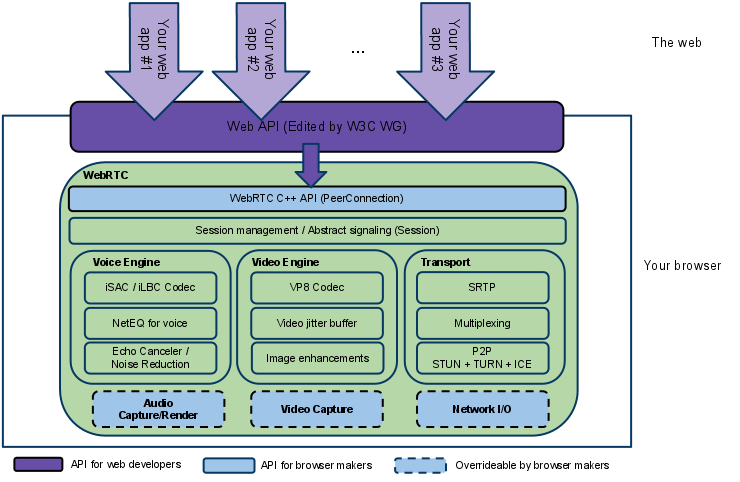
\includegraphics[keepaspectratio=true, width=\textwidth]{images/webrtcArchitecture}\caption{WebRTC architecture (from \url{webrtc.org})}
  \label{fig:webrtcArchitecture}
\end{figure}

\section{WebRTC: Signaling}
\label{sec:webrtc_signaling}
WebRTC uses \RTCPeerConnection to create a connection between peers and communicate audio and video. In order to establish the connection between them it needs a mechanism to coordinate the communication and to send control messages, a process known as signaling. 

Signaling is used to initialize the connection and exchange three types of information:
\begin{itemize}
	\item\textbf{Session control messages}: to initialize or close communication and report errors.
	\item\textbf{Network configuration}: to the outside world, what is my computer's IP address and port?
	\item\textbf{Media capabilities}: what codecs and resolutions can be handled by my browser and the browser it wants to communicate with?
\end{itemize}
The exchange of information via signaling must have successfully completed before peer-to-peer streaming can begin.

Signaling methods and protocols are not specified by WebRTC: signaling is not part of the \RTCPeerConnection API. The web developer can choose the messaging protocol he/she prefer; in this project, WebSockets have been adopted. The reason why the WebRTC group has made this decision is to avoid redundancy and to maximize compatibility with established technologies~\cite{jsep}.

Let us see an example of how to use \RTCPeerConnection: imagine Alice wants to communicate with Bob. To initialize this process, \RTCPeerConnection has two tasks:
\begin{itemize}
	\item Ascertain local media conditions, such as resolution and codec capabilities.
	\item Get potential network addresses for the application's host, known as candidates. (see Sect.\ref{sec:webrtc_ice})
\end{itemize}

For the first point, the exchange of media configuration information proceeds using an offer/answer mechanism that is called JSEP, JavaScript Session Establishment Protocol~\cite{jsep}. Fig.~\ref{fig:jsep} shows the JSEP architecture: both the caller and callee have to save their local session description taken from the browser and send them through some signaling mechanism, then when they receive the session description of the other they set it as the remote session description. Once the process is finished, they both know the configuration of the peer they want to communicate with.

The entire sequence of steps is the following:
\begin{itemize}
	\item Alice creates an \RTCPeerConnection object.
	\item Alice creates an offer using the \RTCPeerConnection \textit{createOffer()} method.
	\item Alice sets her local description to her offer.
	\item Alice uses a signaling mechanism to send her offer to Bob.
	\item Bob sets his remote description to Alice's offer, so that his \RTCPeerConnection knows about Alice's setup.
	\item Bob create an answer using the \textit{createAnswer()} function.
	\item Bob sets his answer as the local description.
	\item Bob then uses the signaling mechanism to send his answer back to Alice.
	\item Alice sets Bob's answer as the remote session description.
\end{itemize}
Offers and answers are communicated in Session Description Protocol format (SDP) \cite{sdp}, which look like this:
\begin{verbatim}
v=0
o=- 7614219274584779017 2 IN IP4 127.0.0.1
s=-
t=0 0
a=group:BUNDLE audio video
a=msid-semantic: WMS
m=audio 1 RTP/SAVPF 111 103 104 0 8 107 106 105 13 126
c=IN IP4 0.0.0.0
a=rtcp:1 IN IP4 0.0.0.0
a=ice-ufrag:W2TGCZw2NZHuwlnf
a=ice-pwd:xdQEccP40E+P0L5qTyzDgfmW
a=extmap:1 urn:ietf:params:rtp-hdrext:ssrc-audio-level
a=mid:audio
a=rtcp-mux
a=crypto:1 AES_CM_128_HMAC_SHA1_80 inline:9c1AHz27dZ9xPI91YNfSlI67/EMkjHHIHORiClQe
a=rtpmap:111 opus/48000/2
....
\end{verbatim}
Using this format, the offer and answer messages contain all the necessary information to guarantee that the peers can communicate using the same codecs, resolution and other media capabilities. 
Once this process is finished, and they both know the configuration of the other, they use the ICE Framework in order to establish the connection.

\begin{figure}[ht]
  \centering
  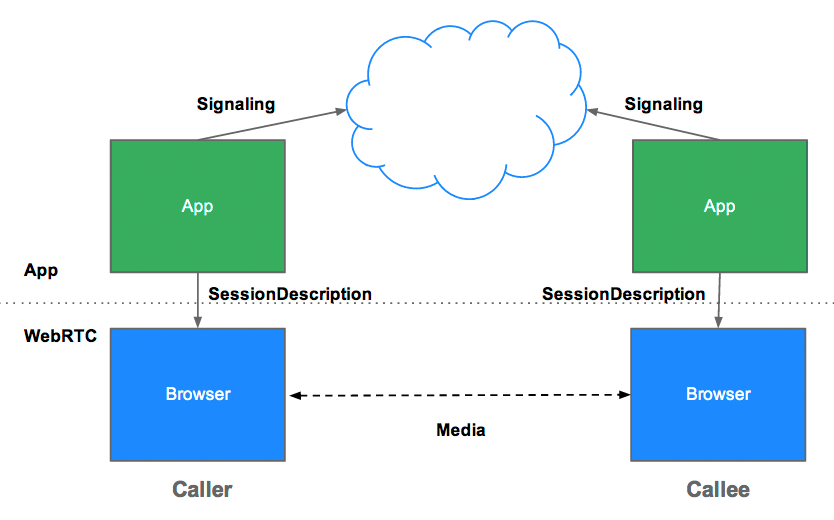
\includegraphics[keepaspectratio=true, width=\textwidth]{images/jsep}\caption{Signaling Diagram}
  \label{fig:jsep}
\end{figure}

\section{WebRTC: ICE Framework}
\label{sec:webrtc_ice}
For metadata signaling, WebRTC applications use an intermediary server, the signaling server, but for actual media and data streaming once a session is established, \RTCPeerConnection attempts to connect clients directly: peer-to-peer. 

In a perfect world, all the nodes are public and they are always reachable. In reality, this is not the case: in fact most devices are behind one or more layers of Network Address Translation (NAT)~\cite{nat}, some have anti-virus software that blocks certain ports and protocols, and many are behind proxies and corporate firewalls. All these configurations make the connection peer-to-peer impossible. However, WebRTC applications can use the \textit{Interactive Connectivity Establishment} (ICE) framework to overcome the complexities of real-world networking. 

ICE tries to find the best path to connect peers. It tries all possibilities in parallel and chooses the most efficient option that works. ICE first tries to make a connection using the host address obtained from a device's operating system and network card; if that fails (which it will for devices behind NATs) ICE obtains an external address using a \textit{Session Traversal Utilities for NAT} (STUN) server, and if that fails, traffic is routed via a \textit{Traversal Using Relays around NAT} (TURN) server\cite{webrtc_infrastructure}. 

In other words, if the direct link fails (so if the peers are behind a NAT), ICE uses the STUN server. Fig.~\ref{fig:stun} shows how it works: the server has one simple task, find the public IP address and port of the peer and send that address back as a response.  This process enables a WebRTC peer to get a publicly accessible address for itself, and then pass that to the other peer via a signaling mechanism, in order to set up a direct link.

If that fails, TURN servers can be used as a fallback. These servers have a conceptually simple task, to relay a stream, but unlike STUN servers, they inherently consume a lot of bandwidth. This is in fact the last chance of the ICE Framework.

Fig.~\ref{fig:turn} represents the complete schema.

\begin{figure}[ht]
  \centering
  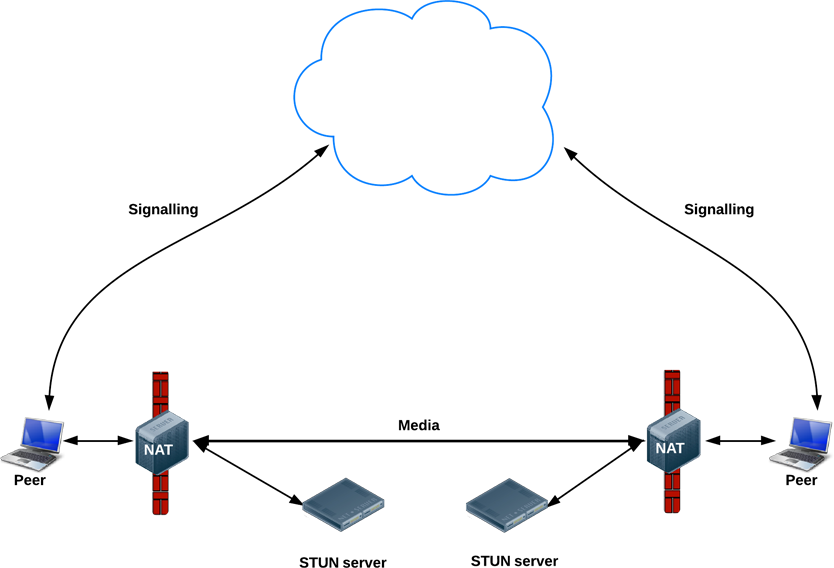
\includegraphics[keepaspectratio=true, width=\textwidth]{images/stun}\caption{Using STUN servers to get public IP:port addresses}
  \label{fig:stun}
\end{figure}

\begin{figure}[ht]
  \centering
  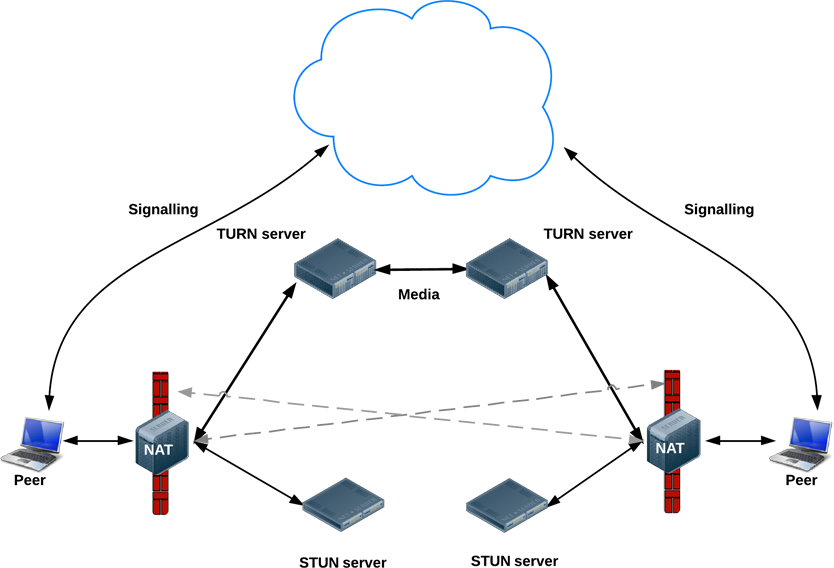
\includegraphics[keepaspectratio=true, width=\textwidth]{images/turn}\caption{The full schema: STUN, TURN and signaling}
  \label{fig:turn}
\end{figure}

The URLs of the STUN and/or TURN servers are (optionally) specified by the WebRTC application in the configuration object that is the first argument of the \RTCPeerConnection constructor. Once \RTCPeerConnection has these information, it uses the ICE framework to work out the best path between peers, working with STUN and TURN servers as necessary. When it find the best solution, it initialize the connection and the peers can start to communicate.

\section{Back to reality: EasyRTC Framework}
\label{sec:easy_tc}
As shown in the previous sections, establishing a connection between two peers in WebRTC is not so simple.
As is often the case with software, with power comes complexity. WebRTC has a learning curve that is likely to hamper its use by web developers. To hide that complexity, Priologic\footnote{A team of Canadian software developers. More information: \url{https://www.priologic.com}} has built the EasyRTC framework.

One of the most important feature of this framework is that, while the WebRTC API requires the developers to implement an involved message passing scheme between clients to establish the peer-to-peer connection, it already provides this schema~\cite{easyrtc} and it is completely hidden from the point of view of the web developers. It is really well documented and there already exists the EasyRTC server (the signaling server) that the nodes will contact in order to register themselves in the network.

EasyRTC is implemented in \textit{Node.js} and it is available for free.

\subsection{EasyRTC Server}
\label{subsec:easyrtc_server}

The main purpose of the server is to serve the requests of ``join the network'' from the nodes, so it is always listening on a specific port and all the nodes have to be able to reach it. Once a node is registered in the network, has an unique identifier that will be valid until it will disconnect. This ID will identify the node within the network, so the other nodes will have to use it in order to contact that specific peer. 

When a node wants to connect to another one, the request pass through this server that will take care of creating the connection between them. Once the connection has been created, the nodes can communicate without passing through the server. 

As explained before, the signaling mechanism is not part of the WebRTC: EasyRTC server by default uses WebSockets\footnote{EasyRTC server by default uses the \emph{socket.io} module. More information: \url{http://socket.io}}. One advantage of this technique is that through the heartbeats (already implemented inside WebSockets) the server knows which nodes are on-line and which ones have disconnected or crashed. In fact every $N$ seconds (by default $N = 25$ seconds), the server sends an heartbeat to the node and if the node does not reply within the heartbeat timeout (by default it is $60$ seconds) it closes the connection with it. We use this technique to capture the failure of a node (it could be crashed or simply disconnected) and send to all the other nodes an advice. If a node was connected to the failed node, it has to replace the broken link with a new one and to do so it contacts the tracker (more information in Sect.\ref{cha:tracker}).

\section{SPOF}
A final issue to be considered is related to the ``Single Point Of Failure'' (SPOF): in our system, if the EasyRTC server crashes or for some reason it is no more reachable from the outside world, no-one can join the network and, especially, no-one can capture the failure of another node (in fact this event is triggered only by the server). Handling this situation is not part of my project, since we start from the assumption that the server is always on-line.

However, there is the possibility to add redundancy in the system, creating more than one server in order to have some of them that acts as backup servers. Then, each node decides which of them to contact, and if for some reasons that server goes down, it connects to another one. In this way the problem is solved, but as explained before this was not the task of the project, so for simplicity we implement only one server and we assume that is always reachable.

      \newpage
      \chapter{Tracker}
\label{cha:tracker}
In the previous sections we saw how a node can initialize a connection to another node using EasyRTC Framework: at the beginning they both have to contact the EasyRTC Server to obtain the ID, and then pass the identifier of the other node to the \textit{connect} function in order to establish the connection. However, EasyRTC does not specify how the nodes have to exchange these identifiers: for this purpose we created a tracker. 

When the nodes bootstrap, they have to contact the EasyRTC Server in order to join the network and then they have to register themselves to the tracker. In this way the latter will eventually have the complete list of the nodes present in the network. When a peer needs to connect to another one (i.e. to replace a broken link):
\begin{itemize}
	\item it asks the tracker a reference of a new node
	\item the tracker chooses an ID at random from the list and it returns it to the peer
	\item the peer analyzes the answer and connects to that ID
\end{itemize}

We use the tracker to provide all nodes with a list of ``initial peers'' to contact in order to start the algorithm (more information in Sect.\ref{cha:wormhole}), to replace the broken links and for all the necessary replacements expected from the algorithm. The main tasks of the tracker are shown in Fig. \ref{fig:tracker}.

In this project the tracker acts like a central server: we only have one tracker for all the nodes, and it has to handle and serve all the requests that derive from the nodes. However, this is not a problem since it has relatively low load (the link replacements are rare) and the algorithm is designed to reduce the number of new network connections created. 

The tracker is hosted on Heroku\footnote{Heroku is a cloud platform that lets companies build, deliver, monitor and scale apps \url{https://www.heroku.com/}} and is implemented in \textit{Node.js}. The nodes contact the tracker using XMLHttpRequest (XHR)\footnote{XMLHttpRequest is an API available to web browser scripting languages such as JavaScript that is used to send HTTP or HTTPS requests to a web server and load the server response data back into the script} and then they parse the response to obtain what they asked.

\begin{figure}[ht]
  \centering
  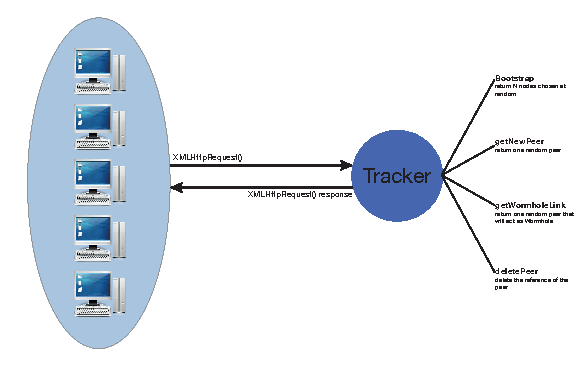
\includegraphics[keepaspectratio=true, width=\textwidth]{images/tracker}\caption{The main tasks of the tracker}
  \label{fig:tracker}
\end{figure}

      \newpage
      \cleardoublepage
      \chapter{Wormhole Peer Sampling Service}
\label{cha:wormhole}
The Wormhole Peer Sampling Service (WPSS)\cite{wormhole} is an algorithm written by Roberto Roverso, Jim Dowling and Mark Jelasity published in 2013. It has been presented in the $13^{th}$ IEEE International Conference on Peer-to-Peer Computing. In the original paper it has been proved, compared to the state of the art at that time, that it has the same levels of samples' freshness  of the other peer sampling services while the connection establishment rate is decreased by one order of magnitude. Another important feature is that it is a NAT-aware protocol, meaning that it handles situations in which some peers are behind NATs or firewall.

In the next sections we are going to see the reasons why these previous aspects might benefit our purpose, and how the algorithm really works.

\section{Peer Sampling Service}
\label{sec:pss}
A peer sampling service (PSS) is a service that runs on all the nodes in a distributed system and provides them with a uniform random sample of live nodes from all nodes in the system, where the sample size is typically much smaller than the system size. 

The reason beyond this service is that, while in the past we had that the network was relatively small and all the nodes had the full view of it (it was almost a static network), now this is not the case anymore: in fact a general distributed system like a peer-to-peer system contains a lot of peers which can join, leave or crash at any time. In this system, having a complete view of the network could be useless or even impossible, so the peer sampling service provides a list of ``fresh'' nodes which reflects the peers known by the node inside the network.

A PSS can be implemented as a centralized service \cite{spotify}, using gossip protocols \cite{gossip_protocol} or random walks \cite{rw}. Gossip-based PSSes have been the most widely adopted solution, as centralized PSSes are expensive to run reliably, and random walks are only suitable for stable networks \cite{rw}. However, in the Internet, where a high percentage of nodes are behind NATs, these traditional gossip-based PSSes become biased. Nodes cannot establish direct connections to nodes behind NATs (private nodes), and private nodes become under-represented in partial views, while nodes that do support direct connectivity, public nodes, become over-represented in partial views\cite{gozar}. 

So to overcome the problem, a new class of NAT-aware gossip-based PSSes have appeared to be able to generate uniformly random node samples even for systems with a high percentage of private nodes, that is, nodes that reside behind a NAT and/or firewall.

State of the art NAT-aware gossip protocols, such as Gozar \cite{gozar} and Croupier\cite{croupier}, require peers to frequently establish network connections and exchange messages with public nodes, nodes that support direct connectivity, in order to build a view of the overlay network. However, in commercial P2P applications such as Spotify \cite{spotify}, P2P-Skype \cite{skype} and as we saw in Sect. \ref{sec:webrtc_api} Google’s WebRTC, establishing a connection is a relatively complex and costly procedure. First of all because privacy is a concern, all new connections require peers to authenticate the other party with a secure server and to setup an encrypted channel. Another reason is that establishing a new connection may involve coordination by a helper service, for instance, to work around connectivity limitations that are not captured by NAT detection algorithms, e.g. using STUN Servers (Sect. \ref{sec:webrtc_ice}). 

In \cite{wormhole} they show that WPSS can provide the same level of freshness of samples as the state of the art in NAT-aware PSSes \cite{croupier} but with a connection establishment rate that is one order of magnitude lower. This, without sacrificing the desirable properties of a PSS for the Internet, such as robustness to churn, NAT-friendliness and local randomness of samples.

\section{WPSS: the algorithm}
\label{sec:wpss_algorithm}
The main idea behind WPSS is that the service is separated into two layers. The bottom layer consists of a stable base overlay network that should be NAT-friendly, with private nodes connecting to public nodes, while public nodes connect to one another. The number of links in the base overlay is fixed at bootstrap-time and it is maintained during all the duration of the algorithm using the tracker (see Sect. \ref{cha:tracker}) to replace the broken links with new ones.

On top of that there is the Wormhole overlay: every node periodically connects to a public node selected randomly from the base overlay (but not necessarily a neighbour). These links to random public nodes are called wormholes: each node systematically places samples of itself on nodes in the neighbourhood of their wormhole. 

Fig. \ref{fig:overlay} shows this mechanism: in the bottom layer, the stable base overlay, there are private nodes connected to public nodes, and public nodes connected to one another; the upper layer, the wormhole overlay, shows a node with its wormhole placing samples of itself in the neighbourhood.

\begin{figure}[ht]
  \centering
  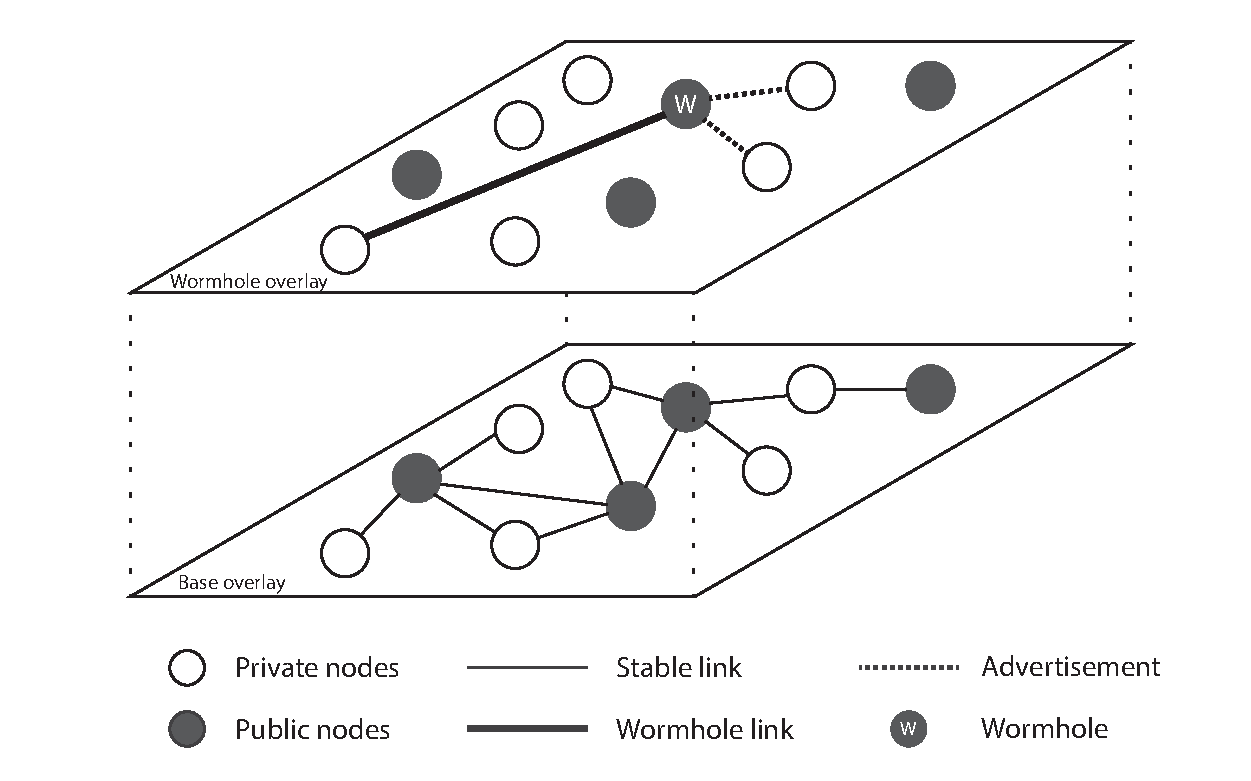
\includegraphics[keepaspectratio=true, width=\textwidth]{images/overlay.pdf}\caption{The difference between the two overlays}
  \label{fig:overlay}
\end{figure}

In other words, when the nodes start they ask the tracker the reference of $N$ random public nodes: that will be their base overlay. Then, they periodically disseminate (push) advertisements of themselves over a small number of hops traversing the wormhole link and they place it at the node where this (typically short) walk terminates.

As explained before, a wormhole link points to a public node in the system that is selected independently at random. In WPSS every node discovers such a random public node to act as its wormhole, and every node only has one wormhole active at any given point in time. A new network connection will be created only when a wormhole is traversed for the first time by an advertisement. The wormhole is then reused for a few subsequent advertisements from the same initiator node, in which case no new network connection needs to be established. This makes it possible to decrease the number of new links established.

The very first time an advertisement reaches the wormhole, it can be placed at the public node as a new sample. However, if the public node already has a sample from the initiator node, then the advertisement will start a random walk over the base overlay until it either reaches a node that does not already have a sample from the initiator node or it reaches a given time-to-live (TTL)\cite{wormhole}.

So, the first time a node will send the advertisement to its wormhole will create a link to it and it will place a sample first at that public node unless it already has an advertisement from the initiator. However, the reuse of the wormhole causes advertisements to continue, allowing them to also finish at private nodes, as private nodes are connected to public nodes over the base overlay. 

When a wormhole is reused by an advertisement, the expected number of hops the advertisement will have to take increases, as it needs to reach a node that does not already have a sample from the initiator node. To counteract this, the WPSS defines a ``wormhole renewal period'' as a parameter for creating new wormholes, enabling users to control how frequently new network connections will be created. We will see in Sect. \ref{cha:evaluation} that tuning this parameter is very important. 


\begin{algorithm}[H]
  \SetKwProg{Upon}{upon}{ do}{end}
  \SetKwProg{Every}{every}{ do}{end}

  \Upon{wormholeFailure}{
  	$wormhole \leftarrow tracker.getNewWormhole()$\;
    $connect(wormhole)$
  }

  \Upon{baseOverlayFailure}{
  	$peer \leftarrow tracker.getNewPeer()$\;
  	$connect(peer)$
  }

  \Every{$\Delta_{wh}$ = wormholeTimeout}{
    $disconnect(wormhole)$\;
  	$wormhole \leftarrow tracker.getNewWormhole()$\;
    $connect(wormhole)$\;
  }

  \Every{$\Delta$ = adTimeout}{
  	$ad \leftarrow createAd()$\;
  	$ad.hops \leftarrow 1$\;
  	$sendAdToWormhole(wormhole, ad)$\;
  }

  \Upon{receivedAd(ad)}{
  	\If{ad.hop = getTTL() $\mid\mid$ acceptAd(ad)}{
  		view.addAd(ad)
  	}\Else{
  		$neighbour \leftarrow getMetropolisHastingsNeighbour(baseOverlay)$\;
  		$ad.hop \leftarrow ad.hop + 1$\;
  		$sendAd(j, ad)$\;
  	}
  }

 \caption{Wormhole peer sampling}
\end{algorithm}

In \textbf{Algorithm 1} there is the pseudo-code of the WPSS. The algorithm runs on all the peers (private and public) in the same way and contains three event-handlers and two timers. 

The event-handlers are: \textit{wormholeFailure}, \textit{baseOverlayFailure} and \textit{receivedAd}. The first two capture the failure of a node (respectively the wormhole and a node present in the base overlay). In these cases the node asks the tracker a reference of a new wormhole/node and it connects to it. The \textit{receiveAd} will be explained later.

Then we have two timers: the wormhole renewal timer $\Delta_{wh}$ that triggers the generation of a new wormhole. In the function, the node disconnects from the old wormhole, it asks the tracker a new one and it connects to it. The other timer $\Delta$ is the rate at which advertisements are published. This timer triggers the sending of one advertisement over the local wormhole. In fact in the function the node creates a new advertisement setting the appropriate parameters (i.e. hop) and it sends it to its wormhole.

Finally the most important function: the \textit{receiveAd}. This function is triggered when a node receives an advertisement: the task is to check if it has to consume it (hence adding it to its view) or it has to forward it. 

The check is performed in two steps: first of all it looks if the TTL of the advertisement is reached, in such a case the node will necessary have to consume it; otherwise it checks if the sample is already contained in the view of the node, in this case it has to forward it. On top of that the \textit{acceptAd} method makes sure that every node consumes advertisements at the same rate, namely one advertisement in each $\Delta$ time period. The reason is that the public nodes will receive a lot of advertisements in a period (because the degree of these nodes are much higher than the private ones, and also because they probably are the wormholes of some private nodes), while the private nodes instead will receive few of them. This check is performed only on the public nodes, and it controls if the node has already consumed an advertisement in the period, in such a case it has to forward it, otherwise it consumes it. We will demonstrate in Sect. \ref{cha:evaluation} that the \textit{acceptAd} method successfully balances advertisements over public and private nodes.

If the node does not consume the advertisement, it sends it to another node using the Metropolis-Hastings transition probabilities over the (random, stable) base network\cite{metropolis}.  Let $d_i$ denote the degree of node \textit{i}, that is, the number of neighbors of node \textit{i}. The implementation of GetMetropolisHastingsNeighbor works as follows. First, we select a neighbor \textit{j} with uniform probability, that is, with probability $1/d_i$. Then, we return \textit{j} with probability $min(d_i /d_j , 1)$, otherwise we return node \textit{i} itself, that is, the advertisement will visit \textit{i} again\cite{wormhole}.

      \newpage
      \chapter{Project Design}
\label{cha:design}
We implemented and tested the project in a real environment and also in simulation. WebRTC APIs are web browser APIs, meaning that they can only work in a browser session. So we developed a first version of the \ac{WPSS} that works in the browser, and tested it with few nodes (100) using Google Chrome\footnote{Google Chrome is a free-ware web browser developed by Google} as browser. Then, in order to test it in a bigger environment we used a simulator. Both versions are implemented using the framework \textbf{Hivejs-Framework} provided by the creator of the algorithm, the Hive Streaming\footnote{Hive Streaming provides network solutions for media distribution and performance analysis. Started as a spin-off in 2007 from the Swedish Institute for Computer Science and the Royal Institute of Technology in Stockholm, the company maintains a strong focus on research and development. \url{https://www.hivestreaming.com}} company. This framework is written in Typescript\footnote{TypeScript is a typed superset of JavaScript that compiles to plain JavaScript. \url{http://www.typescriptlang.org}}, and it enabes us to choose if we want to run the project on browser or directly in \textit{Node.js} simulating a lot of instances. 


\section{Project Architecture}
\label{sec:arch}
At bootstrap-time, the node contacts the EasyRTC Server (Sect.~\ref{subsec:easyrtc_server}) to join the network. Then, it needs a way to build the base overlay with a fixed number of nodes, so it has to register itself to a tracker (Sect.~\ref{cha:tracker}), which it will return the list of the nodes that it has to contact. The tracker is also used to replace the broken links with new ones. In all the other cases, the peers communicate between each other without the help of an external server. The schema with all the steps is shown in Fig.~\ref{fig:project_architecture}.

\begin{figure}[ht]
  \centering
  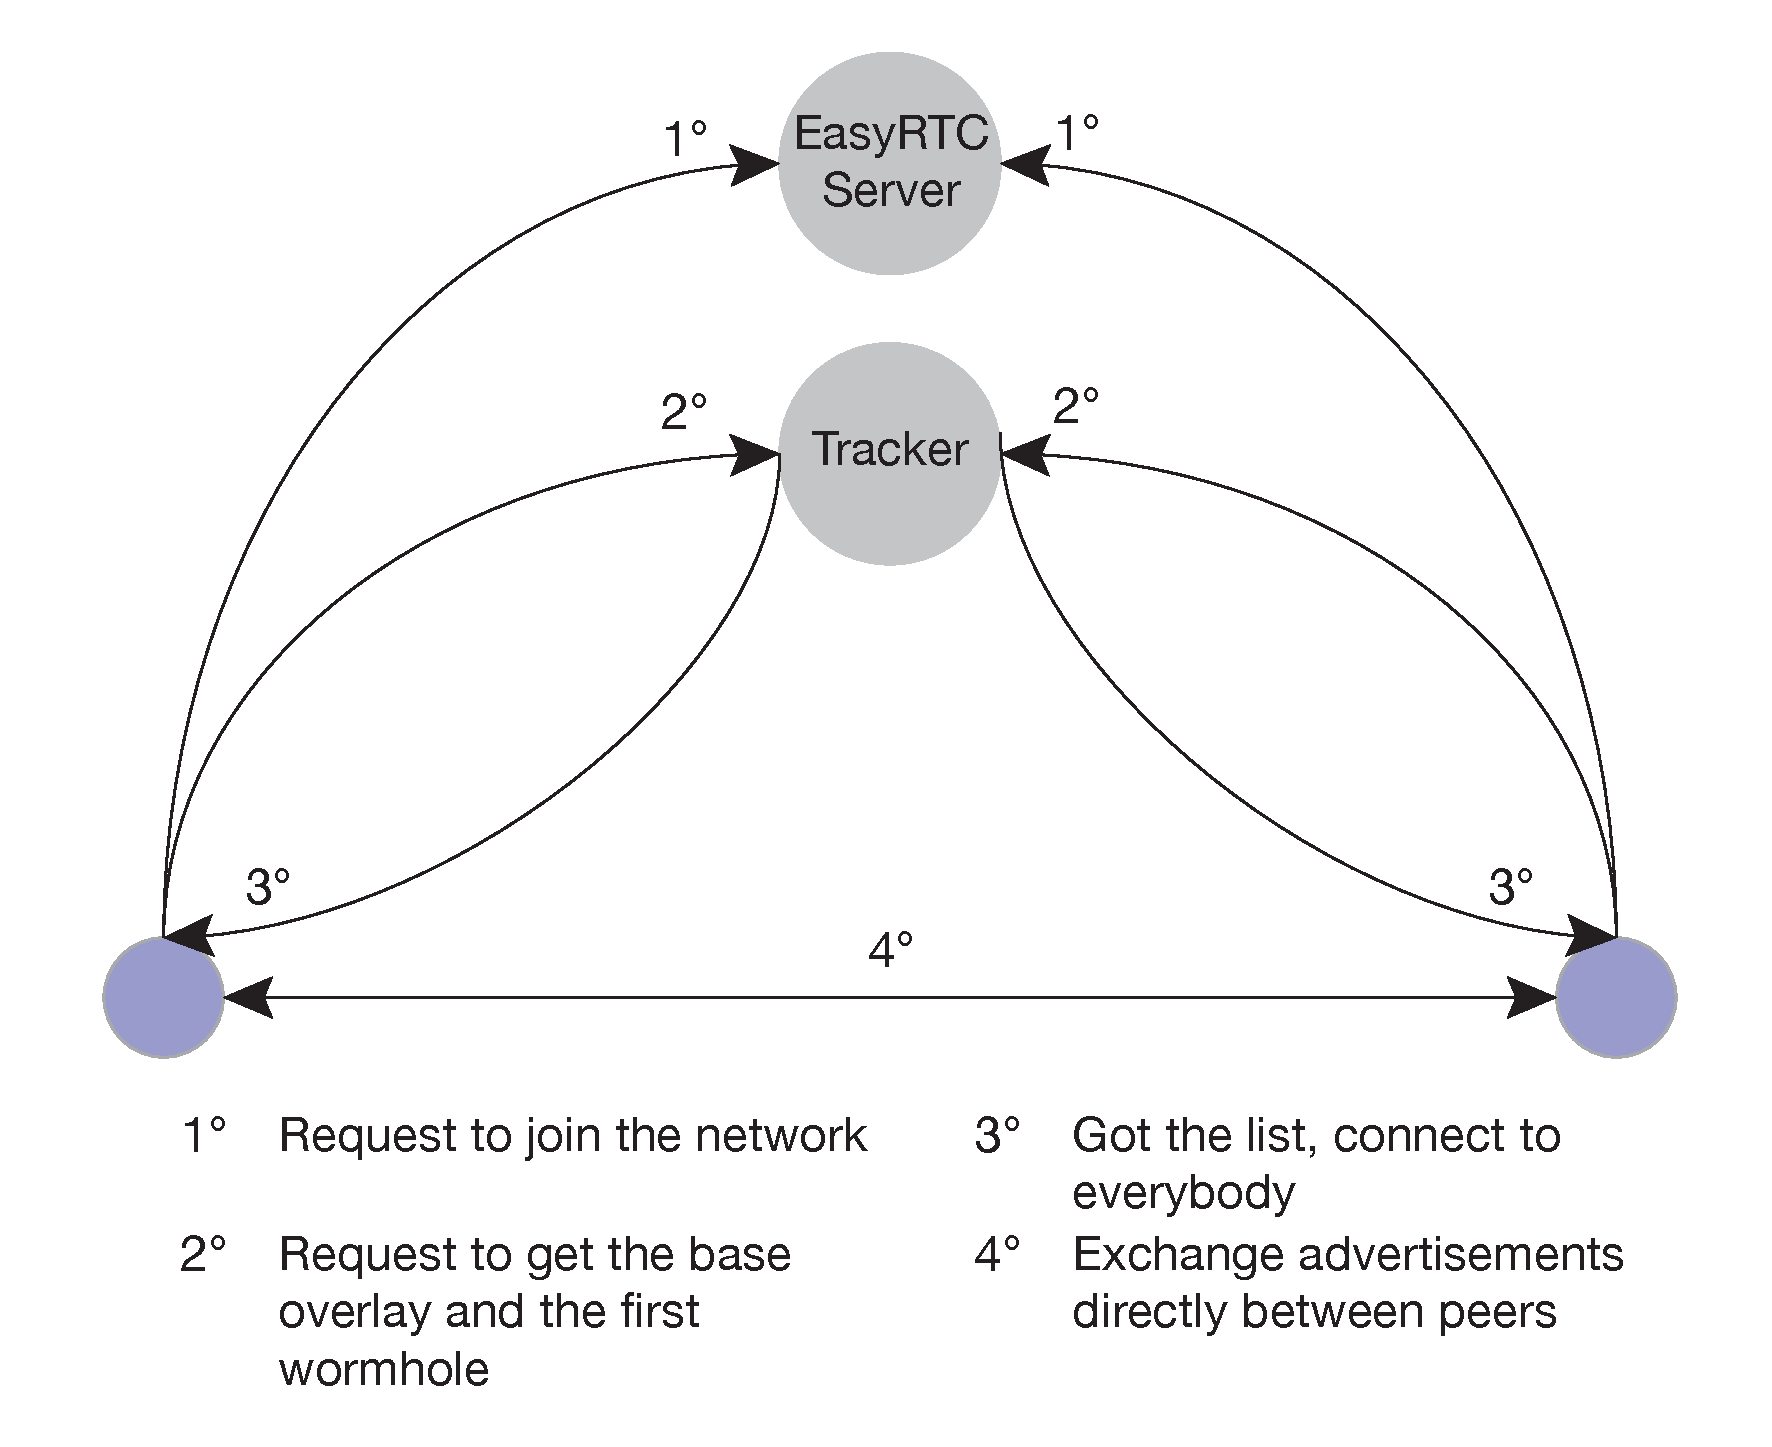
\includegraphics[keepaspectratio=true, width=\textwidth]{images/project_architecture}\caption{The architecture of the project, with the initial steps the nodes have to accomplish}
  \label{fig:project_architecture}
\end{figure}


\section{Node.js Modules}
\label{sec:modules}
The Hivejs-Framework has a WebRTC module for handling peer-to-peer connections which, as explained in Sect.\ref{sec:easy_tc}, is EasyRTC. Then we used a lot of other modules, the most important ones are:

\begin{itemize}
	\item \textbf{Browserify}: with browserify we can use some core \textit{Node.js} modules and many of the thousands modules on npm in our browser-side code
	\item \textbf{Grunt}: it is a task runner, we use it to compile, optimize and ``browserify'' our code. More information at \url{http://gruntjs.com}
	\item \textbf{Inversify}: Inversify is a lightweight (4KB) pico inversion of control (IoC) container for TypeScript and JavaScript applications
	\item \textbf{Q}: a library for promises, more information at \url{https://www.npmjs.com/package/q}
	\item \textbf{Fs}: we use this module only in simulation to write and save the logs of the nodes on local files.
\end{itemize}

The project in order to work correctly needs \textit{Node.js} version 0.12.5, \textit{npm} version 2.11.2 and \textit{Typescript} version 1.7.3.

\section{Special Tools}
We used a lot of tools to simplify the testing phase but also the implementation. One of the most important is NetworkX\footnote{\url{https://networkx.github.io}}, a Python language software package for the creation, manipulation, and study of the structure of complex networks. We used this tool to periodically draw the graphs of the network, in order to have a better representation of the overlays and to check the correctness of the implementation. 
      \newpage
      \cleardoublepage
      %!TEX root = spadini_davide.tex

\chapter{Evaluation}
\label{cha:evaluation}
We now want to evaluate our implementation of the WPSS algorithm, and compare what we obtain with the original papers~\cite{wormhole} in order to confirm or contest their results. We tested our implementation both in deployment and in simulation, however due to the low number of nodes in the real environment we report only the results obtained in simulation. We want to show that our implementation provides the desirable PSS properties, such as fresh samples, randomness, and low cost in a real environment, but also we want to test robustness under different level of churn.

The structure is shown in Fig.~\ref{fig:overlay}, the base overlay is a random undirected graph that is also NAT-friendly, where private nodes are connected to public nodes, and public nodes are connected to one another. The bootstrap service component provides addresses of random public nodes that are used to build the base overlay and to create wormholes. It is implemented as a central server, the tracker. The base overlay service strives to keep the overlay connected repairing broken links, thus, maintaining a fixed number of outgoing links at each node. Every node maintains 20 links to random public nodes, however these links are bidirectional, so the effective average degree is 40. 

We set $TTL = 100$. As discussed in~\cite{wormhole} and also as we will see later, WPSS messages will always terminate much sooner in most practical settings, so the TTL is not a critical parameter.

\section{Experimental Setup}
\label{sec:exp_setup}
For what concerns simulations, we implemented WPSS using the \textbf{Hivejs-Framework-Sim} provided by the Hive Streaming company. It is very configurable, and it allows us to define the network size, the bandwidth of the nodes but also to test the implementation under different level of churn or latency. All experiments are averaged over 4 runs. We applied the same settings as in the original paper, which are: 

\begin{itemize}
	\item the view size (the number of freshest random samples a node remembers) is set to 50
	\item we set $\Delta = 1$ second
	\item we use a scenario of $N = 1000$ nodes that join following a Poisson distribution with a mean inter-arrival time of 100 milliseconds
\end{itemize}

In all simulations 20\% of the nodes is public and 80\% is private, which, according to~\cite{wormhole}, reflects the distribution observed in the commercial deployments of their P2P application.

\section{Freshness}
\label{sec:eval_freshness}
In this experiment we want to measure the freshness of the samples using the average hop count but also the \textit{$90^{th}$} and \textit{$99^{th}$} percentiles. This is the same test reported in~\cite{wormhole}. Fig.~\ref{fig:my_average_hop_count} shows our result, while in Fig.~\ref{fig:paper_average_hop_count} shows their test. As we can see the result is almost identical, this means that our implementation does not alter this property. In the figure we can notice that the average hop count and the $90^{th}$ percentile grow slowly with increasing of $\Delta_{wh}$, which is the wormhole renewal timer, while the $99^{th}$ percentile grows more quickly. This was expected, since the higher the timer, the more nodes the advertisement will need to traverse in order to find a node which does not already have its sample. An important fact to notice is that the \textit{TTL} is never reached, actually in the worst case it is not greater then 20. Another important result here is that the performance is optimal for $\Delta_{wh}$  between about 5 and 10 seconds, as in their result. Given this finding, we set $\Delta_{wh} = 10$ for the remaining experiments, as this value has good freshness (even considering the $99^{th}$ percentile), while the number of new links required is relatively low (a new connection every $10$ rounds of the algorithm). 

\begin{figure}[ht]
  \centering
  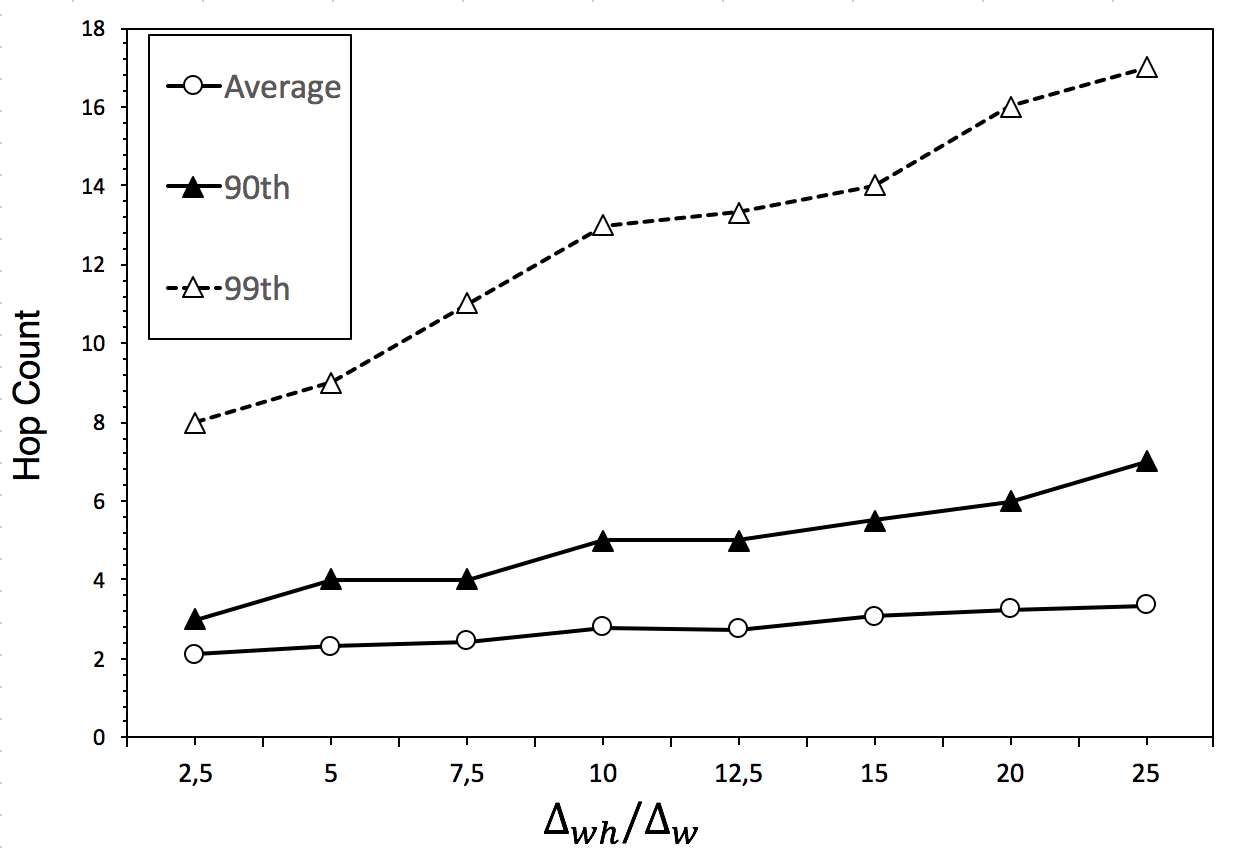
\includegraphics[keepaspectratio=true, width=\textwidth]{images/average_hop_count}\caption{Average hop count}
  \label{fig:my_average_hop_count}
\end{figure}

\begin{figure}[ht]
  \centering
  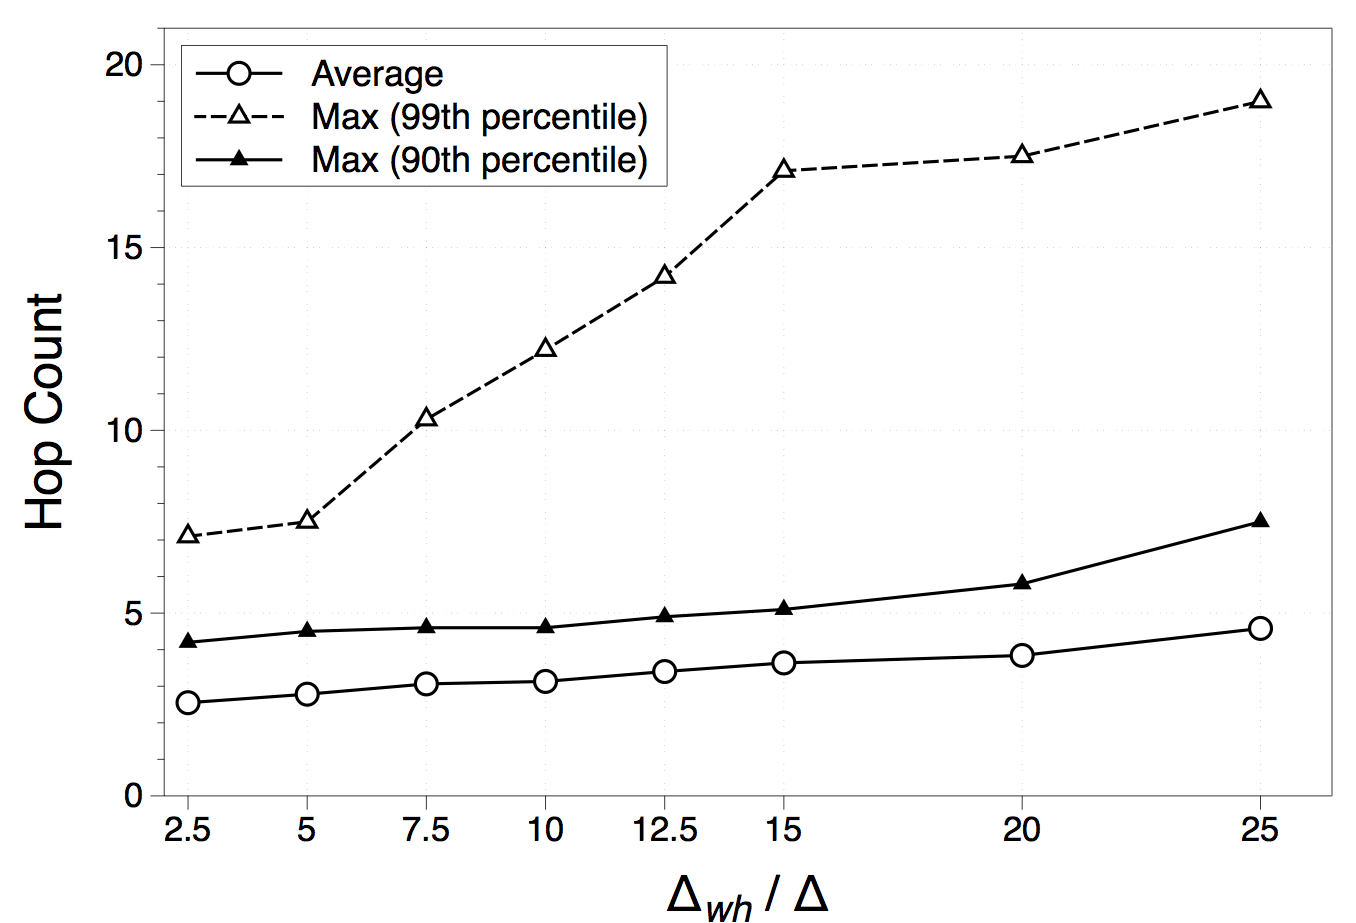
\includegraphics[keepaspectratio=true, width=\textwidth]{images/paper_average_hop_count}\caption{Test of average hop count reported in the paper}
  \label{fig:paper_average_hop_count}
\end{figure}

\section{Randomness}
\label{sec:eval_randomness}
As in \cite{wormhole}, we now want to evaluate the global randomness properties of our system by measuring properties of the WPSS overlay topology, so the upper overlay. This overlay is built connecting to all the samples stored at nodes. In this set of experiments, we measure the in-degree distribution of the WPSS overlay network, its convergence time for different view sizes, and finally its clustering coefficient for different view sizes. In Fig.~\ref{fig:converged_indegree} we can see the converged in-degree distribution. Obviously this result shows that the 95\% of the nodes have an in-degree included between 43 and 55, however there are some nodes that still have a quite large in-degree: these peers are the public nodes, which are initially present in a lot of views, so they have a large in-degree. This result is a little bit different from the original paper, in which they show that all the nodes have an in-degree included between 43 and 60. This is probably due to the environment, because they tried this set of tests in their deployed system, with 12000 nodes and for a long time. 
\begin{figure}[ht]
  \centering
  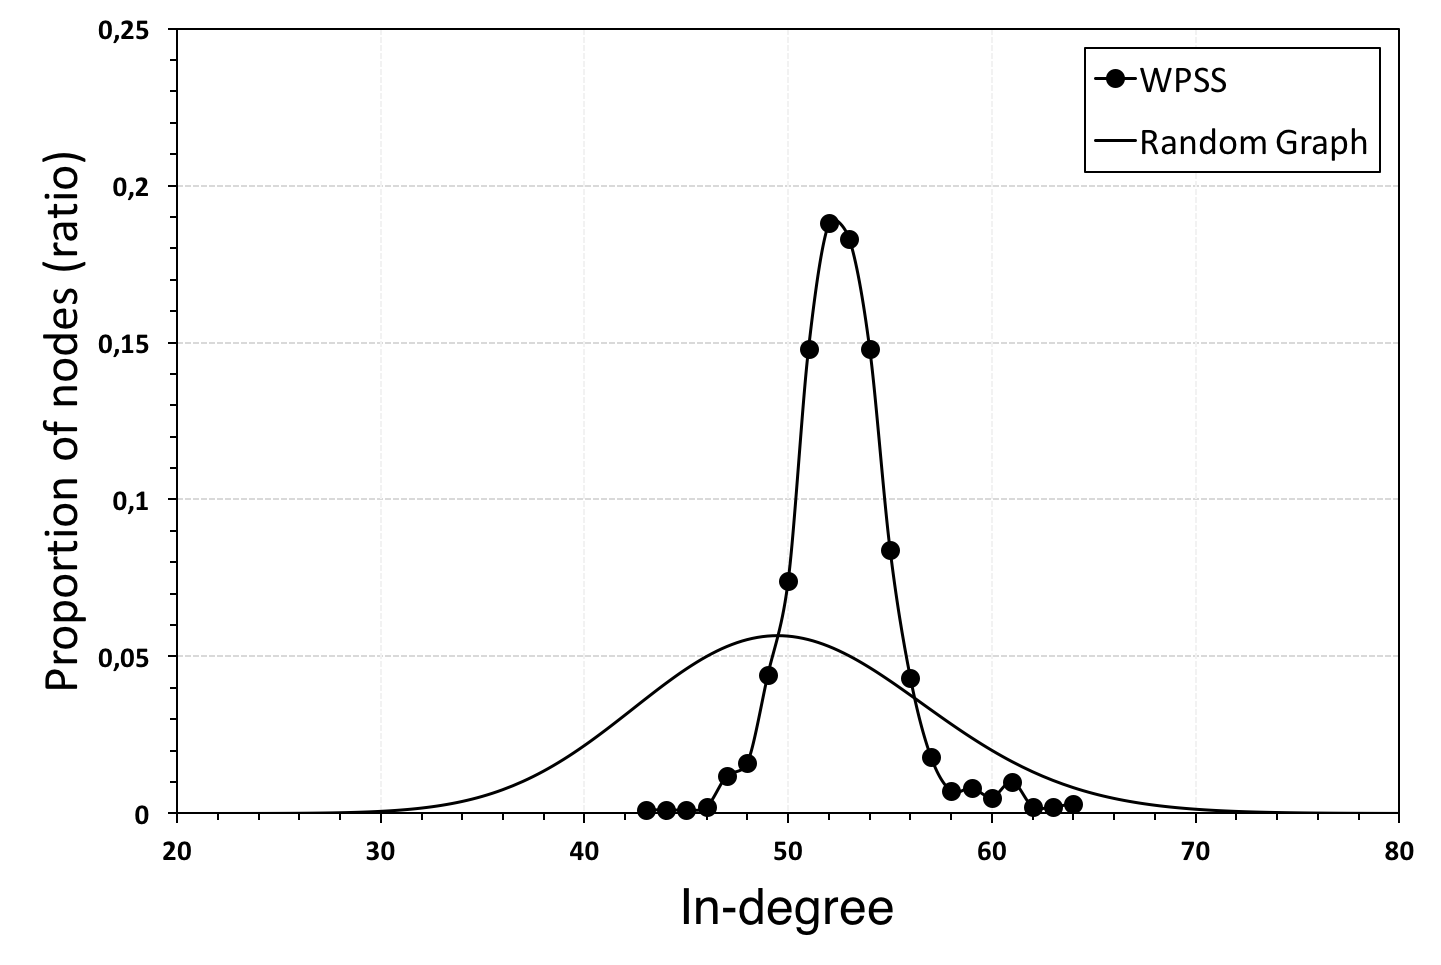
\includegraphics[keepaspectratio=true, width=\textwidth]{images/converged_indegree}\caption{Converged in-degree distribution}
  \label{fig:converged_indegree}
\end{figure}

One interesting fact, that confirms that the problem is not the implementation, is shown in Fig.~\ref{fig:indegree_evolution}: as we can see the in-degree converges to 50 after 4 minutes, and the standard deviation after 8 minutes, which are exactly the same results of the original paper, shown in Fig.~\ref{fig:paper_indegree_evolution}. If we look at this result, we are right to believe that running our implementation for a longer time and with an higher number of nodes could change the result obtained in the converged in-degree graph.

\begin{figure}[ht]
  \centering
  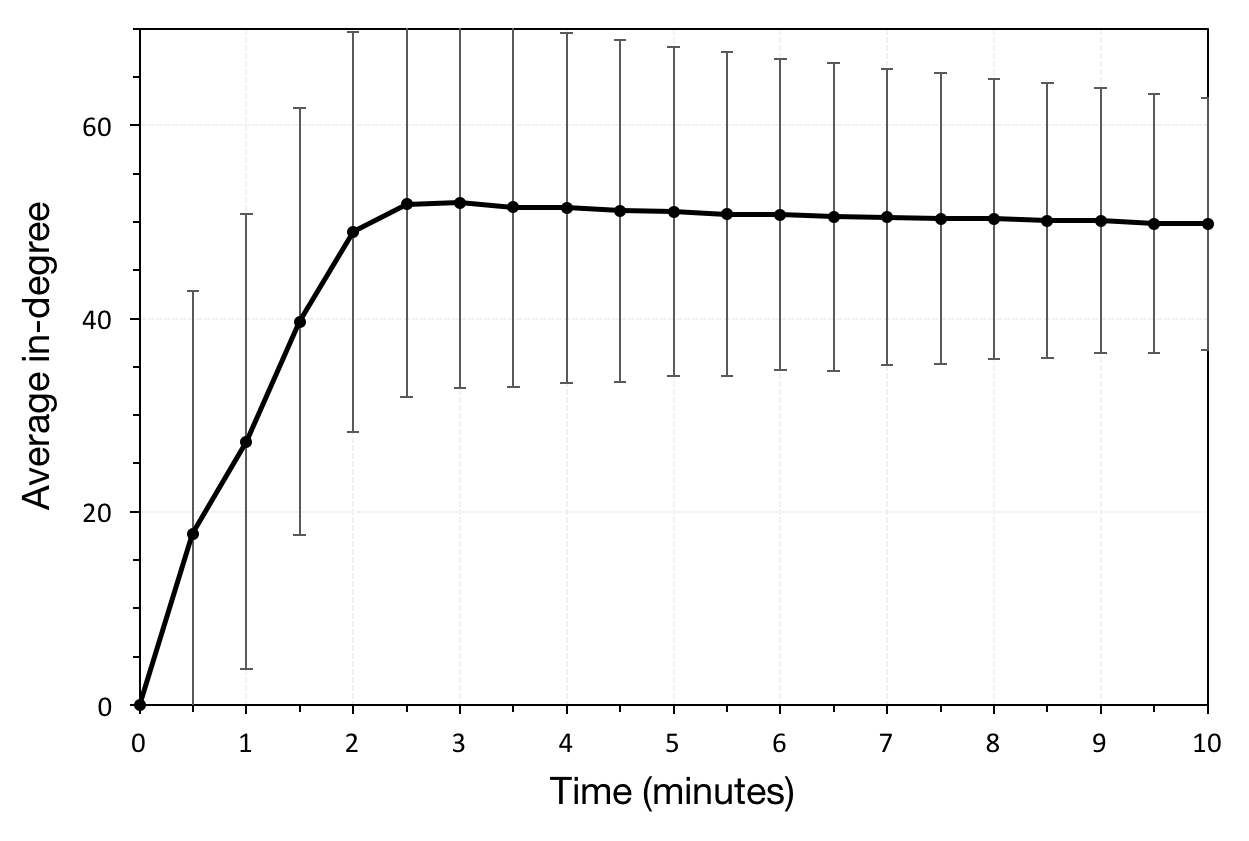
\includegraphics[keepaspectratio=true, width=\textwidth]{images/indegree_evolution}\caption{In-degree evolution over time with error bars}
  \label{fig:indegree_evolution}
\end{figure}

\begin{figure}[ht]
  \centering
  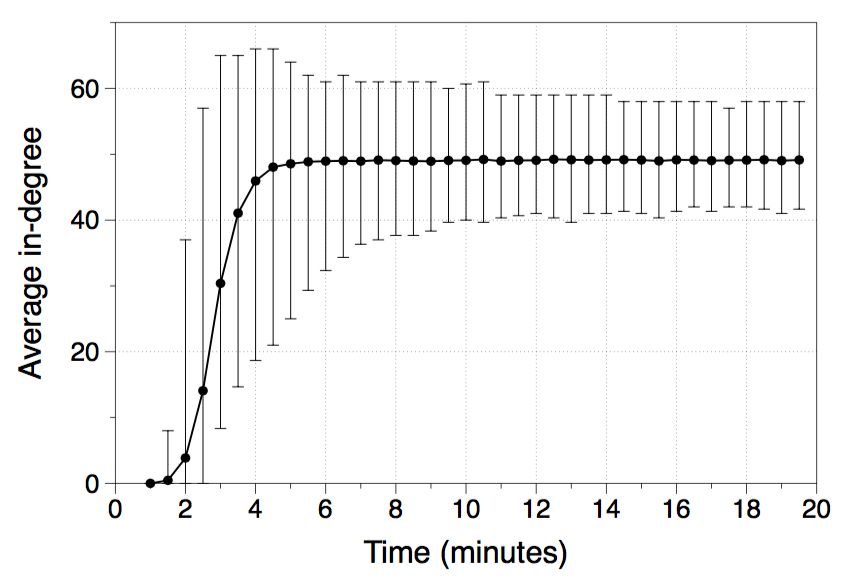
\includegraphics[keepaspectratio=true, width=\textwidth]{images/paper_indegree_evolution}\caption{Test of in-degree evolution reported in the paper}
  \label{fig:paper_indegree_evolution}
\end{figure}

\begin{figure}[ht]
  \centering
  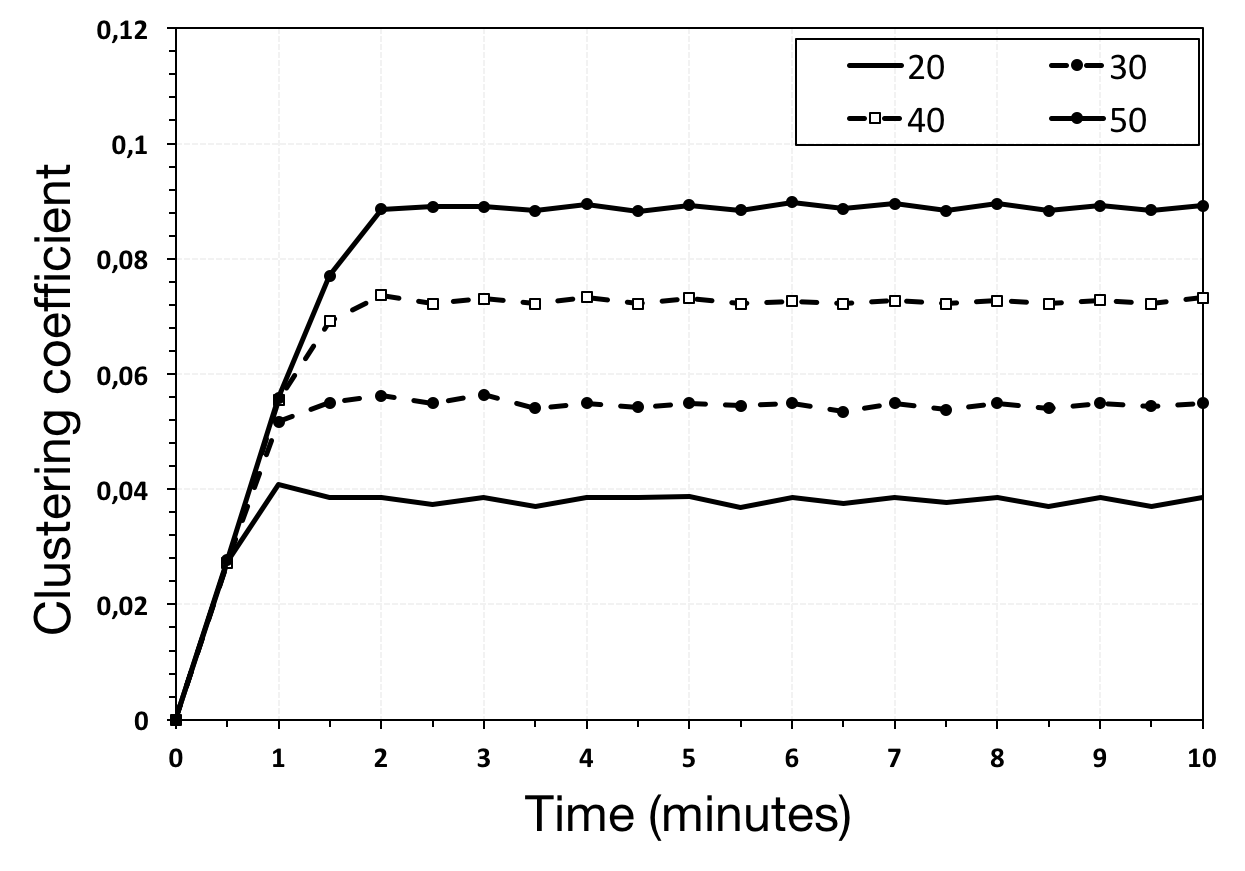
\includegraphics[keepaspectratio=true, width=\textwidth]{images/clustering_coefficient_evolution}\caption{Clustering coefficient evolution for different view sizes}
  \label{fig:clustering_coefficient_evolution}
\end{figure}

Fig.~\ref{fig:clustering_coefficient_evolution} shows the clustering coefficient evolution for different view size, as we can notice it grows with increasing the view size. In fact the higher the view, the higher the number of connections. This result is the same on the original paper. We can also notice that it converges roughly at the same rate as the in-degree.
The last test is shown in Fig.\ref{fig:converged_clustering_coefficient} and it indicates that the clustering coefficient is higher than the one of the random graph by a constant factor, which is due to the fact that WPSS does not guarantee independent samples at nodes that are close in the stable base overlay~\cite{wormhole}.

\begin{figure}[ht]
  \centering
  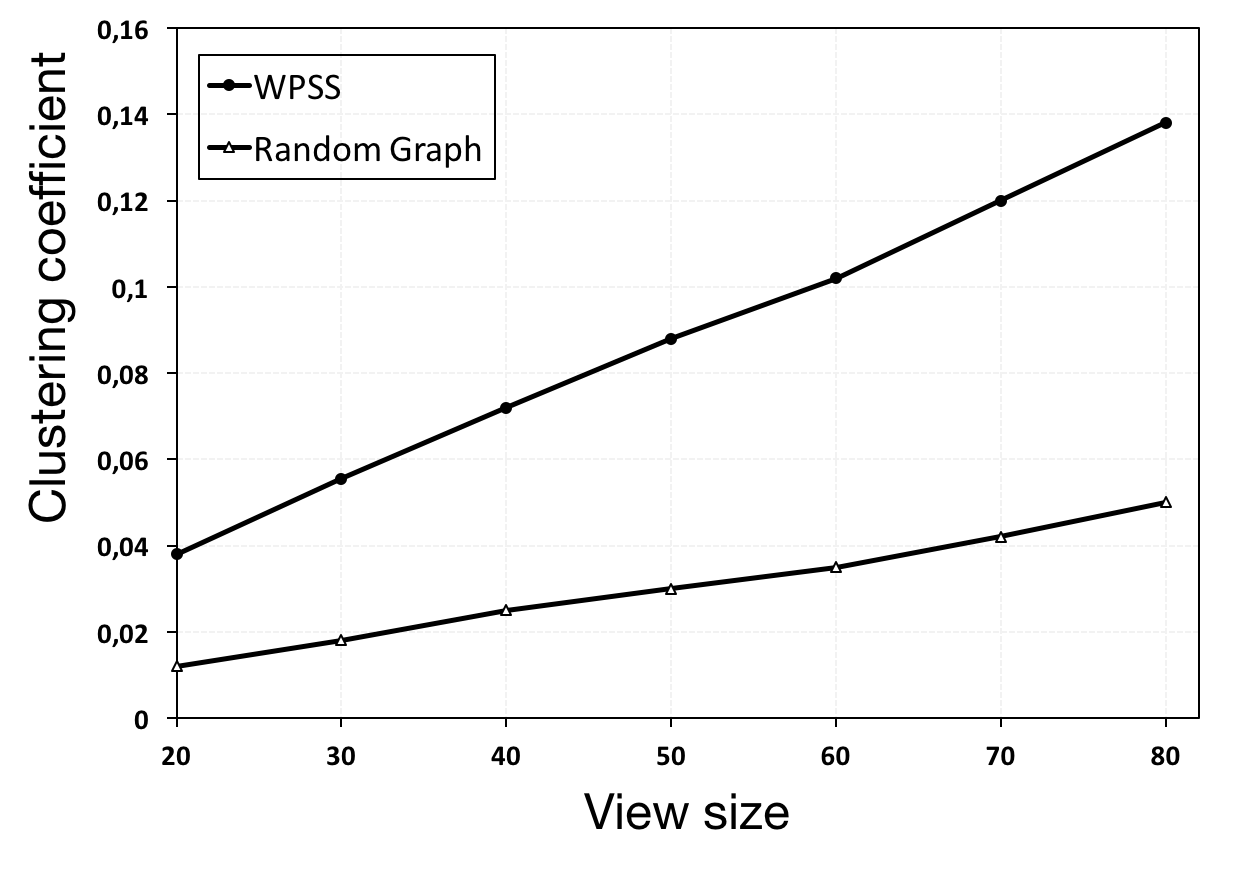
\includegraphics[keepaspectratio=true, width=\textwidth]{images/converged_clustering_coefficient}\caption{Converged clustering coefficient for in- creasing view sizes}
  \label{fig:converged_clustering_coefficient}
\end{figure}

\section{Inter-arrival Time of Advertisements}
\label{sec:interarrivaltime}
In these tests we want to measure the inter-arrival time of the advertisements, so the lapse of time between two consecutive accepted samples. This is an important factor, because the topology is a constraint: in fact the public nodes have a lot of peers connected to them, so they receive more advertisements than the private nodes that are connected only to few nodes. However, the \textit{acceptAd} method takes care of this: it ensures that all the nodes, in average, consume the advertisements at the same rate, namely one in each $\Delta$ period. In Fig.~\ref{fig:average_interarrivaltime} we can observe that the average inter-arrival time of the samples converges to the wormhole period $\Delta$ after about 2 minutes. Except in this time lapse, all the nodes in average consumes one advertisement every $\Delta$, which is exactly the result we were searching. Furthermore, this result is identical to the one shown in the original paper.

Now we want to verify if the \textit{acceptAd} method correctly balances samples across public and private nodes. To do that, we measured the difference inter-arrival time between them. As shown in Fig.~\ref{fig:interarrivaltime_difference} this difference is very low, about $500 ms$ in the worst case in which $\Delta = 6 s$. With $\Delta$ equals to $1s$ or $3s$ the difference is lower, about $100ms$ and $200ms$, so we can confirm that the \textit{acceptAd} method successfully balances the samples between all the nodes, as well as in the original paper.

\begin{figure}[ht]
  \centering
  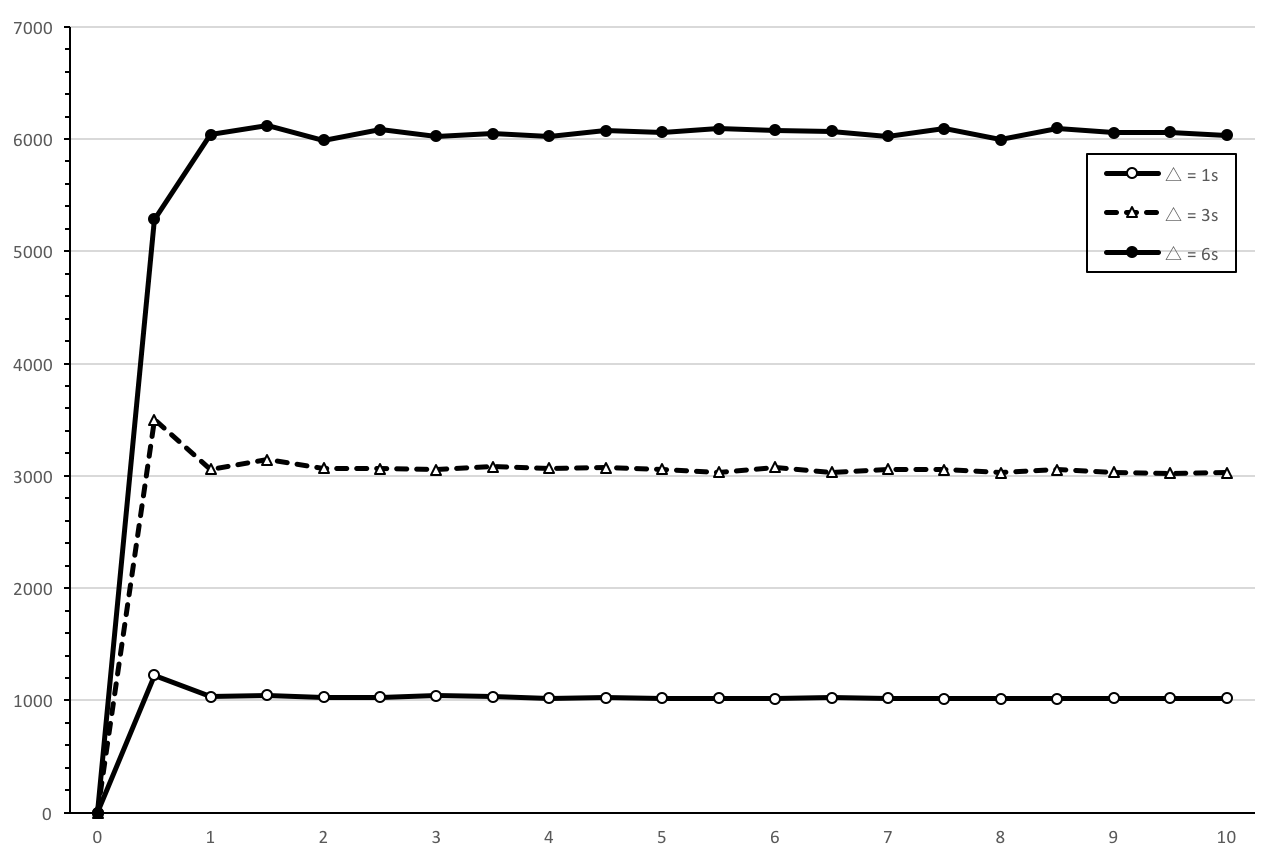
\includegraphics[keepaspectratio=true, width=\textwidth]{images/average_interarrivaltime}\caption{Average inter-arrival time for samples (terminating advertisements) at all peers}
  \label{fig:average_interarrivaltime}
\end{figure}

\begin{figure}[ht]
  \centering
  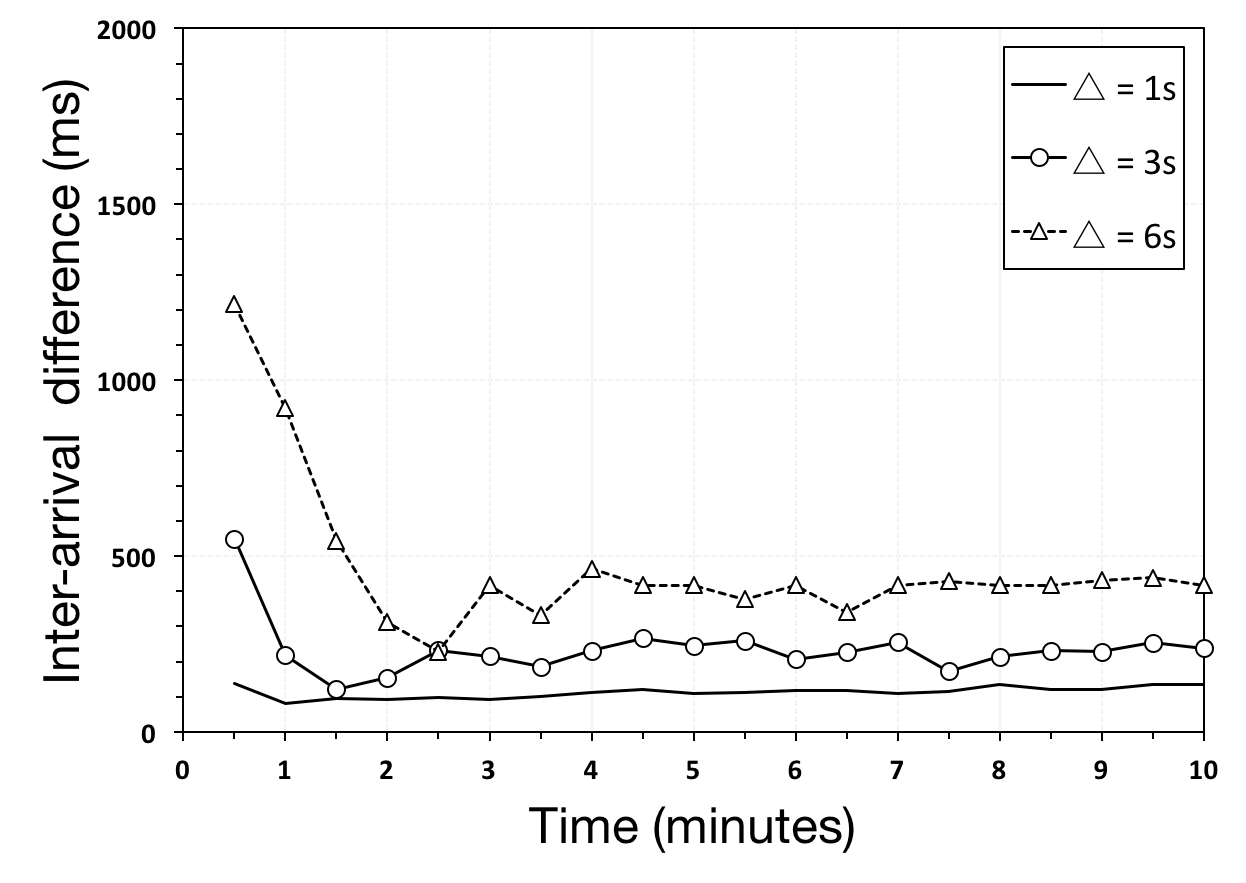
\includegraphics[keepaspectratio=true, width=\textwidth]{images/interarrivaltime_difference}\caption{Difference in inter-arrival time between public and private peers}
  \label{fig:interarrivaltime_difference}
\end{figure}

\section{Robustness to Different Churn Patterns}
\label{sec:robustness}
In this set of experiments we want to test the robustness of our implementation under different levels of churn. We measure the average hop count, as well as the clustering coefficient and the in-degree. In the first three experiments we recreate a flash crowd scenario, in which some nodes join at the beginning and the remaining join at a later point in time. For instance, recalling that $N = 1000$, for a flash crowd scenario of 70\% of the node, 300 nodes join at time $0s$ and 700 nodes join at minute $6.5$. So after this time, the number of nodes stays constant at 1000. In Fig.\ref{fig:average_hop_count_flash_crowd} we can see that the average hop count increases with decreasing the number of nodes that join the system at time 0, in fact an advertisement will have to traverse more nodes in order to reach a peer that does not already have that sample. However at time $6.5$, when all the remaining nodes join the system, the average hop count not only it stabilizes quickly, but it converges to the same value in all the experiments. In Fig.~\ref{fig:paper_average_hop_count_flash_crowd} is shown their result and as we can see they are identical, they also stabilize at the same rate. The next test measures the clustering coefficient in a flash crowd scenario, the expected behavior is similar to the average hop count. As shown in Fig.\ref{fig:average_clustering_coefficient}, this is the case. In fact the clustering coefficient stabilizes quickly and to the same rate when all the nodes join the network. Finally, Fig.\ref{fig:average_indegree} shows the average in-degree of the nodes. As we can see after two minutes in all the experiments the nodes have in average the same in-degree, then it drops significantly at time $6.5$, this is in fact expected since a majority of the nodes join the network with in-degree equals to 0. However, it recovers quickly (about $1.30$ minutes later) and it converges to 50 in all the experiments.

In the next set of experiments we measure the robustness of our implementation in case of catastrophic failures, that is, when a large number of peers leaves the system at a single instant in time. All the nodes join the system at time $0$, we wait for the overlay to stabilize and then we fail a fixed percentage of nodes at time $5$ minutes. We expect that the algorithm recovers quickly and also that all the nodes remain connected, even in the worst case scenario where 80\% of the peers leave the system. In Fig.\ref{fig:average_hop_count_failures} we can notice that all the experiments has the same average hop count until time $5$ minutes, then it increases with increasing of failures. This is expected given the large number of broken links to detect and repair for both the base and wormhole overlays. Notice that the network remains connected even when 80\% of the nodes fail. Fig.~\ref{fig:average_clustering_coefficient_failures} shows the evolution of the clustering coefficient: it increases with increasing of failures, since there are less nodes in the network and they are much more connected between each other. One important experiment in case of massive failures is to measure the average number of dead links in the views of the peers. What we want to obtain is a system which detect and replace the broken links as fast as possible. Fig.~\ref{fig:average_dead_links} shows the result: at time $5$ the number of dead links increases (obviously the higher the failures, the higher the number of dead links), however after just one minute all the broken links are successfully deleted from the views (even in the worst case where 80\% of the nodes fail), and the average number returns equals to zero. This result is even better of the one shown in the original paper, because the time employed by them to replace the links is two minutes, we do it in half time. This is probably due the fact that we use a tracker, which has high availability and it responds to all the nodes immediately, while they use the random walks, so they need more time to find a node and establish a new network connection.

\begin{figure}[ht]
  \centering
  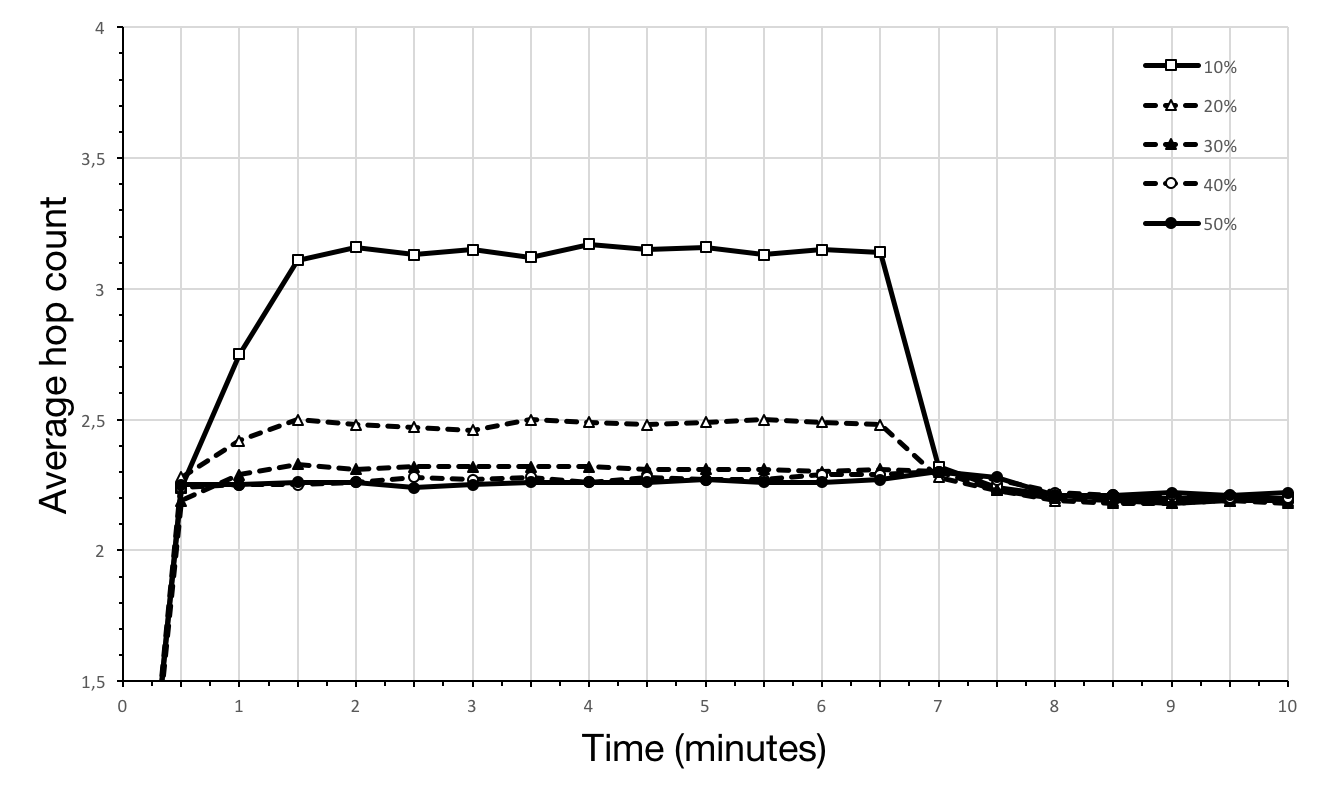
\includegraphics[keepaspectratio=true, width=\textwidth]{images/average_hop_count_flash_crowd}\caption{Average hop count}
  \label{fig:average_hop_count_flash_crowd}
\end{figure}

\begin{figure}[ht]
  \centering
  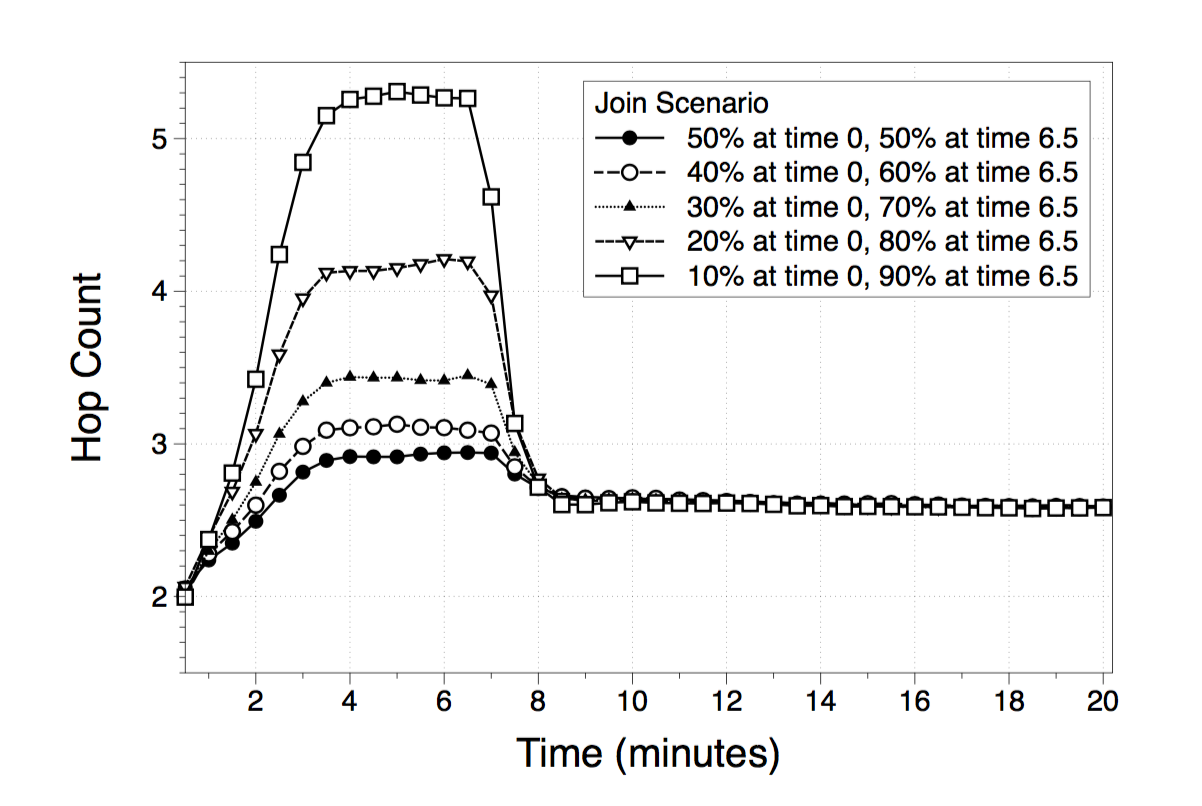
\includegraphics[keepaspectratio=true, width=\textwidth]{images/paper_average_hop_count_flash_crowd}\caption{Test of the average hop count in a flash crowd scenario reported in the paper}
  \label{fig:paper_average_hop_count_flash_crowd}
\end{figure}

\begin{figure}[ht]
  \centering
  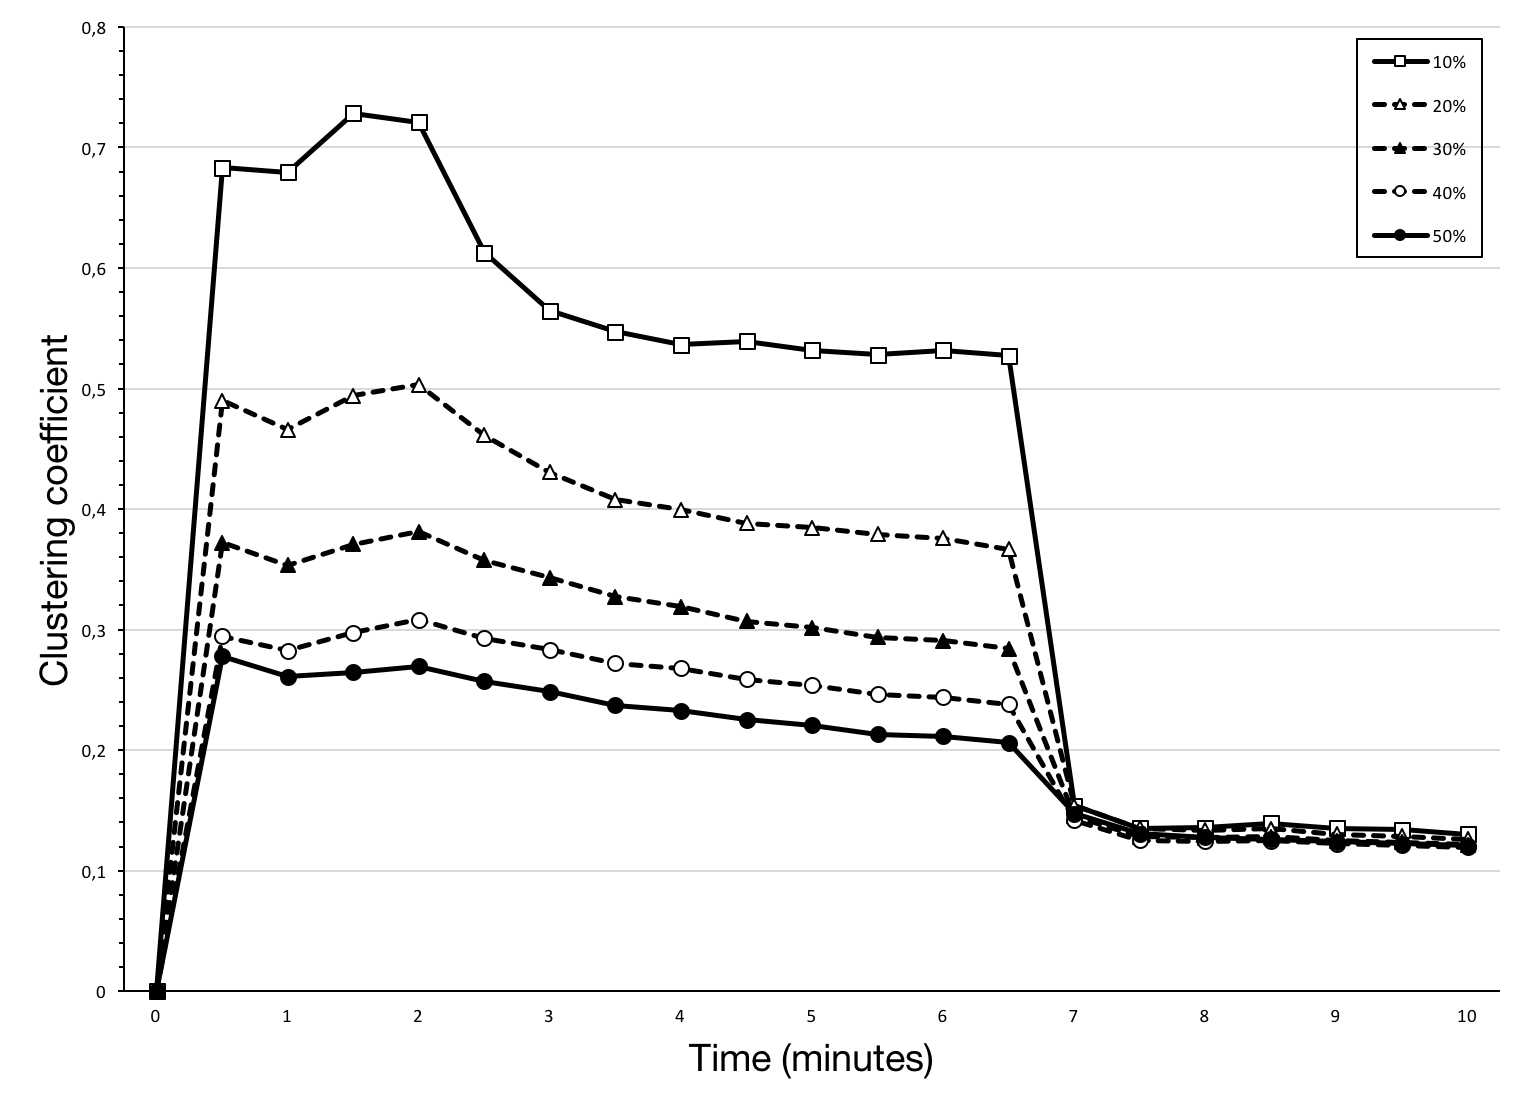
\includegraphics[keepaspectratio=true, width=\textwidth]{images/average_clustering_coefficient}\caption{Average clustering coefficient}
  \label{fig:average_clustering_coefficient}
\end{figure}

\begin{figure}[ht]
  \centering
  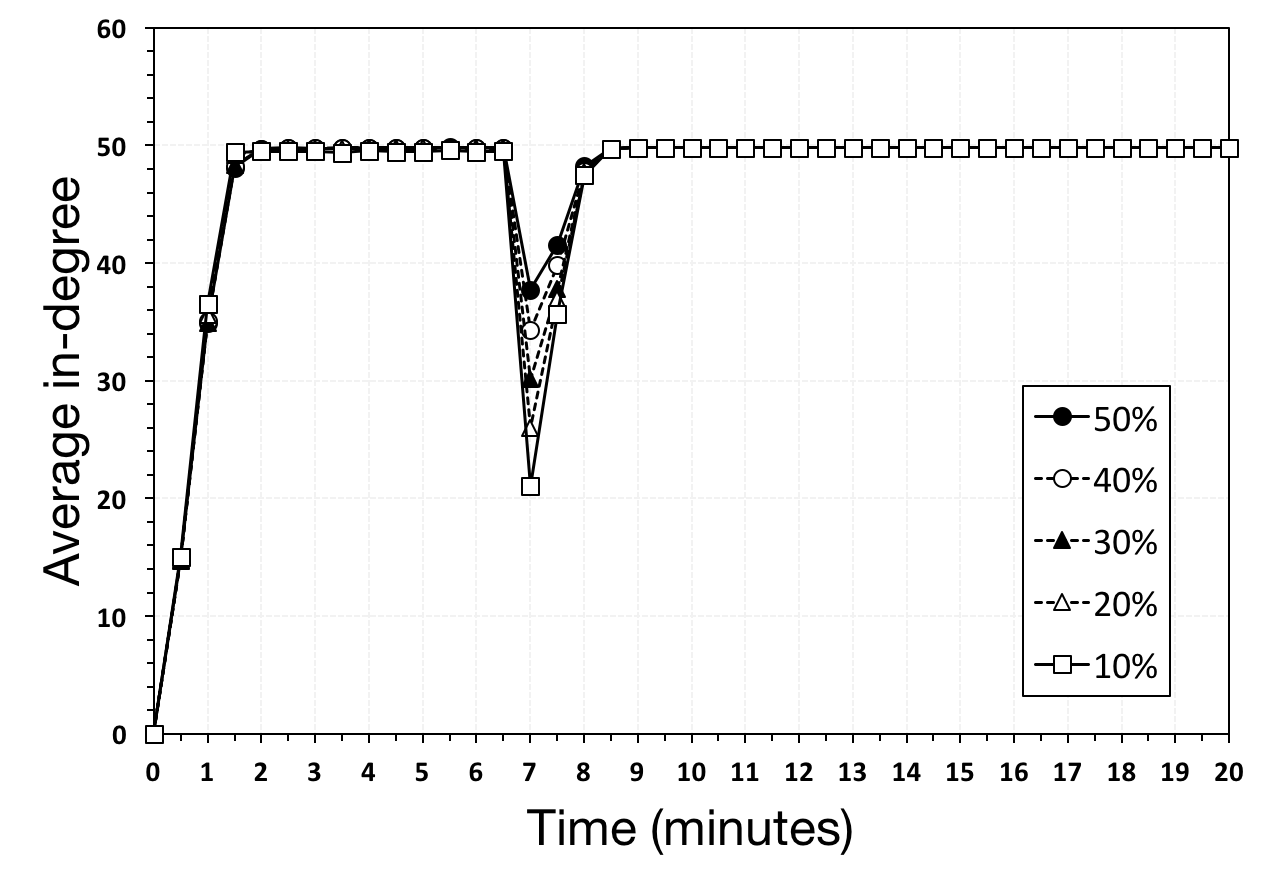
\includegraphics[keepaspectratio=true, width=\textwidth]{images/average_indegree}\caption{Average in-degree}
  \label{fig:average_indegree}
\end{figure}

\begin{figure}[ht]
  \centering
  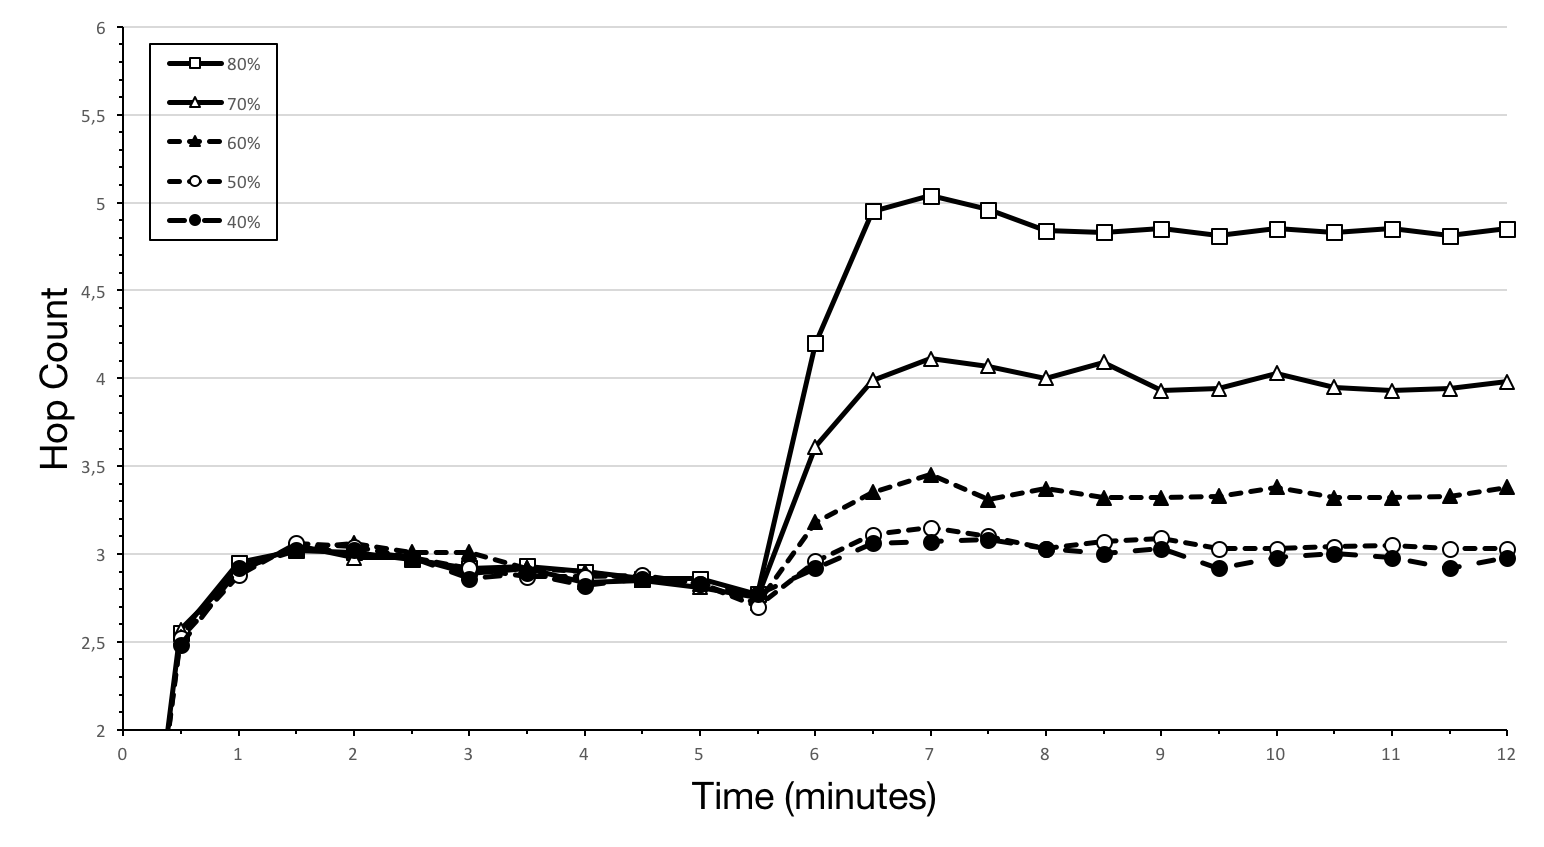
\includegraphics[keepaspectratio=true, width=\textwidth]{images/average_hop_count_failures}\caption{Average hop count}
  \label{fig:average_hop_count_failures}
\end{figure}

\begin{figure}[ht]
  \centering
  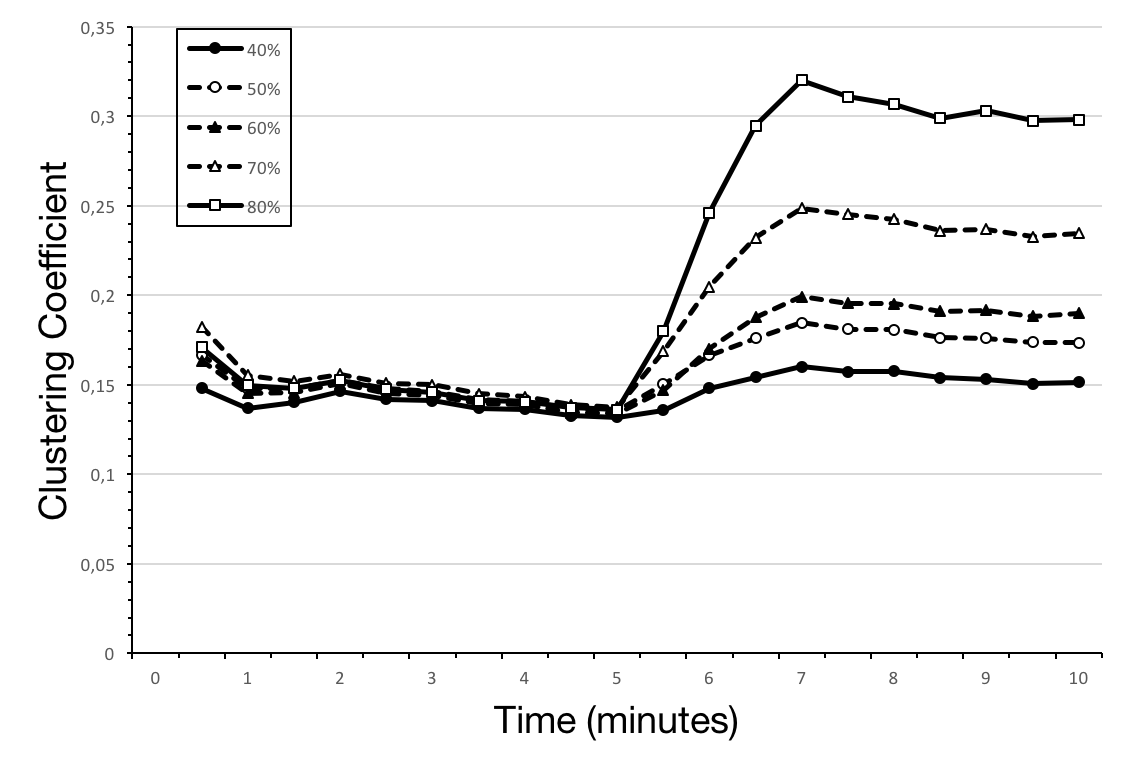
\includegraphics[keepaspectratio=true, width=\textwidth]{images/average_clustering_coefficient_failures}\caption{Average clustering coefficient}
  \label{fig:average_clustering_coefficient_failures}
\end{figure}

\begin{figure}[ht]
  \centering
  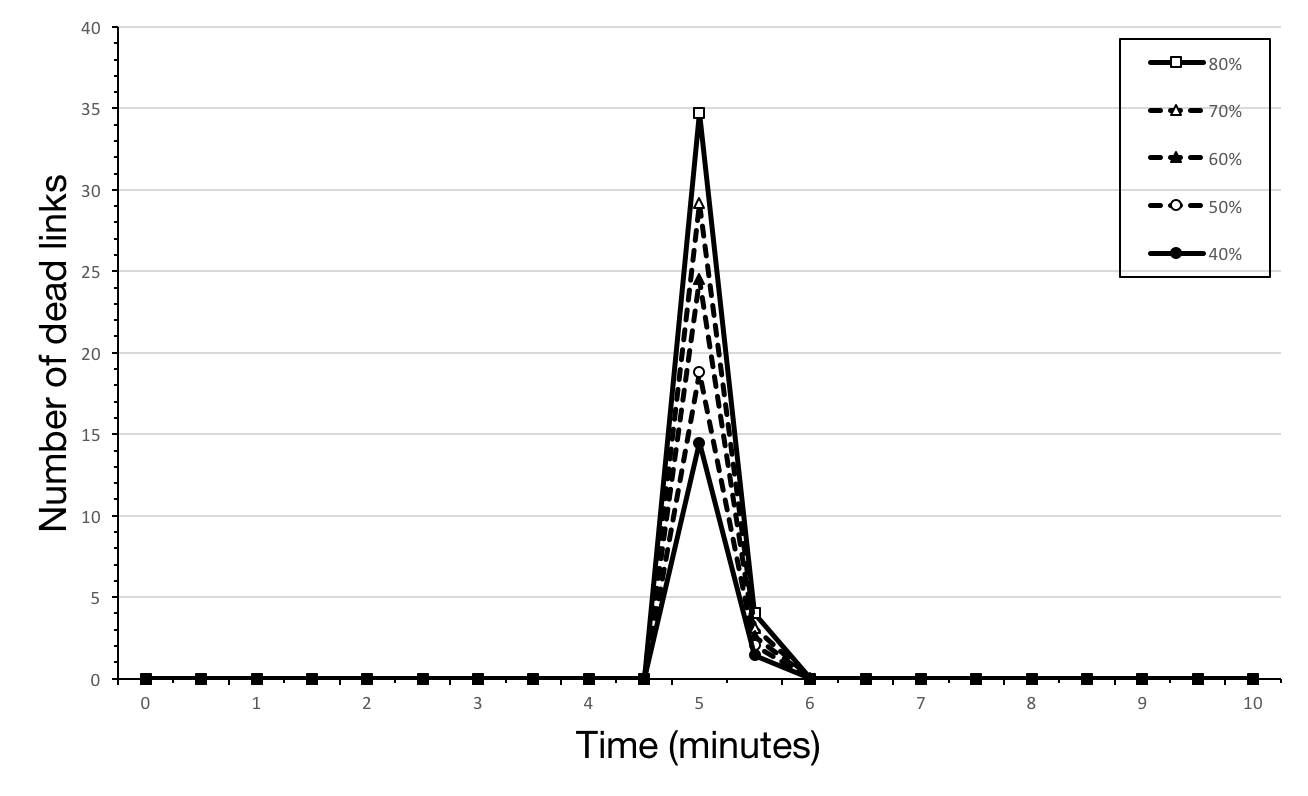
\includegraphics[keepaspectratio=true, width=\textwidth]{images/average_dead_links}\caption{Average number of dead links in view}
  \label{fig:average_dead_links}
\end{figure}

      %\input{capitolo4}
      
      
    \endgroup


    % bibliografia in formato bibtex
    %
    % aggiunta del capitolo nell'indice
    \addcontentsline{toc}{chapter}{Bibliografia}
    % stile con ordinamento alfabetico in funzione degli autori
    \bibliographystyle{plain}
    \bibliography{biblio}

%%%%%%%%%%%%%%%%%%%%%%%%%%%%%%%%%%%%%%%%%%%%%%%%%%%%%%%%%%%%%%%%%%%%%%%%%%
%%%%%%%%%%%%%%%%%%%%%%%%%%%%%%%%%%%%%%%%%%%%%%%%%%%%%%%%%%%%%%%%%%%%%%%%%%
%% Nota
%%%%%%%%%%%%%%%%%%%%%%%%%%%%%%%%%%%%%%%%%%%%%%%%%%%%%%%%%%%%%%%%%%%%%%%%%%
%% Nella bibliografia devono essere riportati tutte le fonti consultate 
%% per lo svolgimento della tesi. La bibliografia deve essere redatta 
%% in ordine alfabetico sul cognome del primo autore. 
%% 
%% La forma della citazione bibliografica va inserita secondo la fonte utilizzata:
%% 
%% LIBRI
%% Cognome e iniziale del nome autore/autori, la data di edizione, titolo, casa editrice, eventuale numero dell’edizione. 
%% 
%% ARTICOLI DI RIVISTA
%% Cognome e iniziale del nome autore/autori, titolo articolo, titolo rivista, volume, numero, numero di pagine.
%% 
%% ARTICOLI DI CONFERENZA
%% Cognome e iniziale del nome autore/autori (anno), titolo articolo, titolo conferenza, luogo della conferenza (città e paese), date della conferenza, numero di pagine. 
%% 
%% SITOGRAFIA
%% La sitografia contiene un elenco di indirizzi Web consultati e disposti in ordine alfabetico. 
%% E’ necessario:
%%   Copiare la URL (l’indirizzo web) specifica della pagina consultata
%%   Se disponibile, indicare il cognome e nome dell’autore, il titolo ed eventuale sottotitolo del testo
%%   Se disponibile, inserire la data di ultima consultazione della risorsa (gg/mm/aaaa).    
%%%%%%%%%%%%%%%%%%%%%%%%%%%%%%%%%%%%%%%%%%%%%%%%%%%%%%%%%%%%%%%%%%%%%%%%%%
%%%%%%%%%%%%%%%%%%%%%%%%%%%%%%%%%%%%%%%%%%%%%%%%%%%%%%%%%%%%%%%%%%%%%%%%%%
    

    \titleformat{\chapter}
        {\normalfont\Huge\bfseries}{Allegato \thechapter}{1em}{}
    % sezione Allegati - opzionale
    \appendix
    % \chapter{Titolo primo allegato}

Lorem ipsum dolor sit amet, consectetur adipiscing elit. Donec sed nunc orci. Aliquam nec nisl vitae sapien pulvinar dictum quis non urna. Suspendisse at dui a erat aliquam vestibulum. Quisque ultrices pellentesque pellentesque. Pellentesque egestas quam sed blandit tempus. Sed congue nec risus posuere euismod. Maecenas ut lacus id mauris sagittis egestas a eu dui. Class aptent taciti sociosqu ad litora torquent per conubia nostra, per inceptos himenaeos. Pellentesque at ultrices tellus. Ut eu purus eget sem iaculis ultricies sed non lorem. Curabitur gravida dui eget ex vestibulum venenatis. Phasellus gravida tellus velit, non eleifend justo lobortis eget. 

\section{Titolo}
Lorem ipsum dolor sit amet, consectetur adipiscing elit. Donec sed nunc orci. Aliquam nec nisl vitae sapien pulvinar dictum quis non urna. Suspendisse at dui a erat aliquam vestibulum. Quisque ultrices pellentesque pellentesque. Pellentesque egestas quam sed blandit tempus. Sed congue nec risus posuere euismod. Maecenas ut lacus id mauris sagittis egestas a eu dui. Class aptent taciti sociosqu ad litora torquent per conubia nostra, per inceptos himenaeos. Pellentesque at ultrices tellus. Ut eu purus eget sem iaculis ultricies sed non lorem. Curabitur gravida dui eget ex vestibulum venenatis. Phasellus gravida tellus velit, non eleifend justo lobortis eget. 

\subsection{Sottotitolo}
Lorem ipsum dolor sit amet, consectetur adipiscing elit. Donec sed nunc orci. Aliquam nec nisl vitae sapien pulvinar dictum quis non urna. Suspendisse at dui a erat aliquam vestibulum. Quisque ultrices pellentesque pellentesque. Pellentesque egestas quam sed blandit tempus. Sed congue nec risus posuere euismod. Maecenas ut lacus id mauris sagittis egestas a eu dui. Class aptent taciti sociosqu ad litora torquent per conubia nostra, per inceptos himenaeos. Pellentesque at ultrices tellus. Ut eu purus eget sem iaculis ultricies sed non lorem. Curabitur gravida dui eget ex vestibulum venenatis. Phasellus gravida tellus velit, non eleifend justo lobortis eget. 


\chapter{Titolo secondo allegato}

Lorem ipsum dolor sit amet, consectetur adipiscing elit. Donec sed nunc orci. Aliquam nec nisl vitae sapien pulvinar dictum quis non urna. Suspendisse at dui a erat aliquam vestibulum. Quisque ultrices pellentesque pellentesque. Pellentesque egestas quam sed blandit tempus. Sed congue nec risus posuere euismod. Maecenas ut lacus id mauris sagittis egestas a eu dui. Class aptent taciti sociosqu ad litora torquent per conubia nostra, per inceptos himenaeos. Pellentesque at ultrices tellus. Ut eu purus eget sem iaculis ultricies sed non lorem. Curabitur gravida dui eget ex vestibulum venenatis. Phasellus gravida tellus velit, non eleifend justo lobortis eget. 

\section{Titolo}
Lorem ipsum dolor sit amet, consectetur adipiscing elit. Donec sed nunc orci. Aliquam nec nisl vitae sapien pulvinar dictum quis non urna. Suspendisse at dui a erat aliquam vestibulum. Quisque ultrices pellentesque pellentesque. Pellentesque egestas quam sed blandit tempus. Sed congue nec risus posuere euismod. Maecenas ut lacus id mauris sagittis egestas a eu dui. Class aptent taciti sociosqu ad litora torquent per conubia nostra, per inceptos himenaeos. Pellentesque at ultrices tellus. Ut eu purus eget sem iaculis ultricies sed non lorem. Curabitur gravida dui eget ex vestibulum venenatis. Phasellus gravida tellus velit, non eleifend justo lobortis eget. 

\subsection{Sottotitolo}
Lorem ipsum dolor sit amet, consectetur adipiscing elit. Donec sed nunc orci. Aliquam nec nisl vitae sapien pulvinar dictum quis non urna. Suspendisse at dui a erat aliquam vestibulum. Quisque ultrices pellentesque pellentesque. Pellentesque egestas quam sed blandit tempus. Sed congue nec risus posuere euismod. Maecenas ut lacus id mauris sagittis egestas a eu dui. Class aptent taciti sociosqu ad litora torquent per conubia nostra, per inceptos himenaeos. Pellentesque at ultrices tellus. Ut eu purus eget sem iaculis ultricies sed non lorem. Curabitur gravida dui eget ex vestibulum venenatis. Phasellus gravida tellus velit, non eleifend justo lobortis eget. 




\end{document}
